This chapter provides the results of the different approaches that have been used during the evaluation phase. First, the results of the Exploration Algorithm are presented. The test cases were all done visually using Python plots as described in section \ref{sec:Visual Verification with Plots}. Second, the results of the Optimization Algorithm are presented. Again, the test cases are outputted visually using Python plots as described in section \ref{sec:Visual Verification with Plots}. Additionally, each track's calculation times and estimated lap times were calculated. In the end, the integration tests with both algorithms are presented using the Simulation Tool.

\section{Exploration Algorithm Specifics} \label{sec:Exploration Algorithm Specifics}
The exploration algorithm tests were done using Python plots. Track information like cone positions and the starting position of the car were loaded from the track files by the \acrlong{tum}. \cite{tumftm_optimization_algoritm} Additionally, each algorithm cycle and the total algorithm calculation time were observed.

Different config parameters for the thresholds had to be loaded for each track for the Exploration Algorithm, as the scale of the tracks were not similar. The different parameters are the starting position of the car on the track, the position distance threshold (maximum distance a newly received cone can have with the car's current position), the cone distance threshold (maximum distance nearby cones can have with the newly received cone, to be considered for triangulation), the cones threshold (minimum number of cones for triangulation) and the edges distance threshold (maximum length an edge can have to be considered for middle point calculation). The default parameters for the Exploration Algorithm are given as follows in table \ref{tab:Default Track Config for Exploration Algorithm}:
\begin{table}[H]
    \centering
    \begin{tabular}{|l|l|l|}
        \hline
        \textbf{Config Parameter}     & \textbf{Value} \\ \hline
        START\_CURRENT\_POSITION      & [0.0, 0.0]     \\ \hline
        POSITION\_DISTANCE\_THRESHOLD & 20 m           \\ \hline
        CONE\_DISTANCE\_THRESHOLD     & 12 m           \\ \hline
        CONES\_THRESHOLD              & 3              \\ \hline
        EDGE\_DISTANCE\_THRESHOLD     & 7 m            \\ \hline
    \end{tabular}
    \caption{Current default track configuration parameters. They are subject to change after further testing.}
    \label{tab:Default Track Config for Exploration Algorithm}
\end{table}

\section{Optimization Algorithm Specifics}
The Optimization Algorithm makes use of many parameters. A GGV diagram (performance envelope) showing the maximum acceleration the car can sustain in any horizontal direction when travelling at any speed. Furthermore, an 'Ax Machines Array' containing an array with the longitudinal acceleration limits by the electrical motors, among other things. The default data for the GGV diagram is shown in table \ref{tab:GGV Diagram}, while the default data for the 'Ax Machines Array' is shown in table \ref{tab:Ax Machines Array}. As both of those have not yet been recorded for the actual race car of \acrshort{zur}, the default data provided by \acrshort{tumftm} has been used.

\begin{table}[H]
    \centering
    \begin{tabular}{|l|l|l|}
        \hline
        \textbf{v\_mps} & \textbf{ax\_max\_mps2} & \textbf{ay\_max\_mps2} \\ \hline
        0.0             & 12.0                   & 12.0                   \\ \hline
        4.0             & 12.0                   & 12.0                   \\ \hline
        8.0             & 12.0                   & 12.0                   \\ \hline
        12.0            & 12.0                   & 12.0                   \\ \hline
        16.0            & 12.0                   & 12.0                   \\ \hline
        20.0            & 12.0                   & 12.0                   \\ \hline
        24.0            & 12.0                   & 12.0                   \\ \hline
        28.0            & 12.0                   & 12.0                   \\ \hline
        32.0            & 12.0                   & 12.0                   \\ \hline
        36.0            & 12.0                   & 12.0                   \\ \hline
        40.0            & 12.0                   & 12.0                   \\ \hline
        44.0            & 12.0                   & 12.0                   \\ \hline
        48.0            & 12.0                   & 12.0                   \\ \hline
        52.0            & 12.0                   & 12.0                   \\ \hline
        56.0            & 12.0                   & 12.0                   \\ \hline
        60.0            & 12.0                   & 12.0                   \\ \hline
        64.0            & 12.0                   & 12.0                   \\ \hline
        68.0            & 12.0                   & 12.0                   \\ \hline
        72.0            & 12.0                   & 12.0                   \\ \hline
    \end{tabular}
    \caption{The supplied GGV diagram (``ggv.csv''), also known as the performance envelope, shows the maximum acceleration the car can sustain in any horizontal direction when travelling at any speed.}
    \label{tab:GGV Diagram}
\end{table}

\begin{table}[H]
    \centering
    \begin{tabular}{|l|l|l|}
        \hline
        \textbf{v\_mps} & \textbf{ax\_max\_machines\_mps2} \\ \hline
        0.0             & 5.3                              \\ \hline
        4.0             & 5.3                              \\ \hline
        8.0             & 5.3                              \\ \hline
        12.0            & 5.3                              \\ \hline
        16.0            & 5.3                              \\ \hline
        20.0            & 5.3                              \\ \hline
        24.0            & 5.3                              \\ \hline
        28.0            & 5.3                              \\ \hline
        32.0            & 5.3                              \\ \hline
        36.0            & 5.3                              \\ \hline
        40.0            & 5.1                              \\ \hline
        44.0            & 5.0                              \\ \hline
        48.0            & 4.6                              \\ \hline
        52.0            & 4.1                              \\ \hline
        56.0            & 3.7                              \\ \hline
        60.0            & 2.7                              \\ \hline
        66.0            & 2.2                              \\ \hline
        72.0            & 1.5                              \\ \hline
    \end{tabular}
    \caption{The supplied ``ax\_max\_machines.csv'', containing an array with the longitudinal acceleration limits by the electrical motors.}
    \label{tab:Ax Machines Array}
\end{table}

Furthermore, additional options have been used with the Optimization Algorithm, those being step size options, spline regression smooth options, velocity profile calculation options, specific optimization problem options, and the general vehicle parameters. Excluding the general vehicle parameters, the set options are:
\begin{itemize}
    \item Step Size options
          \begin{itemize}
              \item Step Size Prep: 1.0 m (used for linear interpolation before spline approximation)
              \item Step Size Reg: 3.0 m (used for spline interpolation after spline approximation during optimization)
              \item Step Size Interp: 2.0 m (used for spline interpolation after optimization)
          \end{itemize}
    \item Spline Regression Smooth options
          \begin{itemize}
              \item K: 3 (order of B-Splines)
              \item S: 10 (smoothing factor ranging from 1.0 to 100.0)
          \end{itemize}
    \item Velocity Profile Calculation options
          \begin{itemize}
              \item Dyn Model Exp: 1.0 (exponents used in the vehicle dynamics model ranging from 1.0 to 2.0)
              \item Conv Filt Window: not used (moving average filter window size for velocity profile)
          \end{itemize}
    \item Optimization Problem Options
          \begin{itemize}
              \item Width Opt: 2.6 m (Vehicle Width for Optimization including Safety Distance)
              \item IQP Iters Min: 3 (minimum number of iterations for IQP)
              \item IQP Curv Error Allowed: 0.01 rad/m (maximum allowed curvature error for IQP)
          \end{itemize}
\end{itemize}

As it goes for the general vehicle parameters, the real specifications of the \acrshort{zur} race car have been provided and are listed in table \ref{tab:ZUR Vehicle Specifications}. The car is shown in figure \ref{fig:ZUR Racecar 2}.
\begin{table}[H]
    \centering
    \begin{tabular}{|l|l|l|}
        \hline
        \textbf{Parameter} & \textbf{Value} & \textbf{Description}           \\ \hline
        V Max              & 30.61 m/s      & Maximal Vehicle Speed          \\ \hline
        Length             & 2.931 m        & Vehicle Length                 \\ \hline
        Width              & 1.663 m        & Vehicle Width                  \\ \hline
        Mass               & 255.0 kg       & Vehicle Mass                   \\ \hline
        Drag Coeff         & 0.3 kg*m2/m3   & Drag Coefficient               \\ \hline
        Curv Lim           & 0.33 rad/m     & Curvature Limit of the Vehicle \\ \hline
    \end{tabular}
    \caption{The vehicle's specifications.}
    \label{tab:ZUR Vehicle Specifications}
\end{table}
\begin{figure}[H]
    \centering
    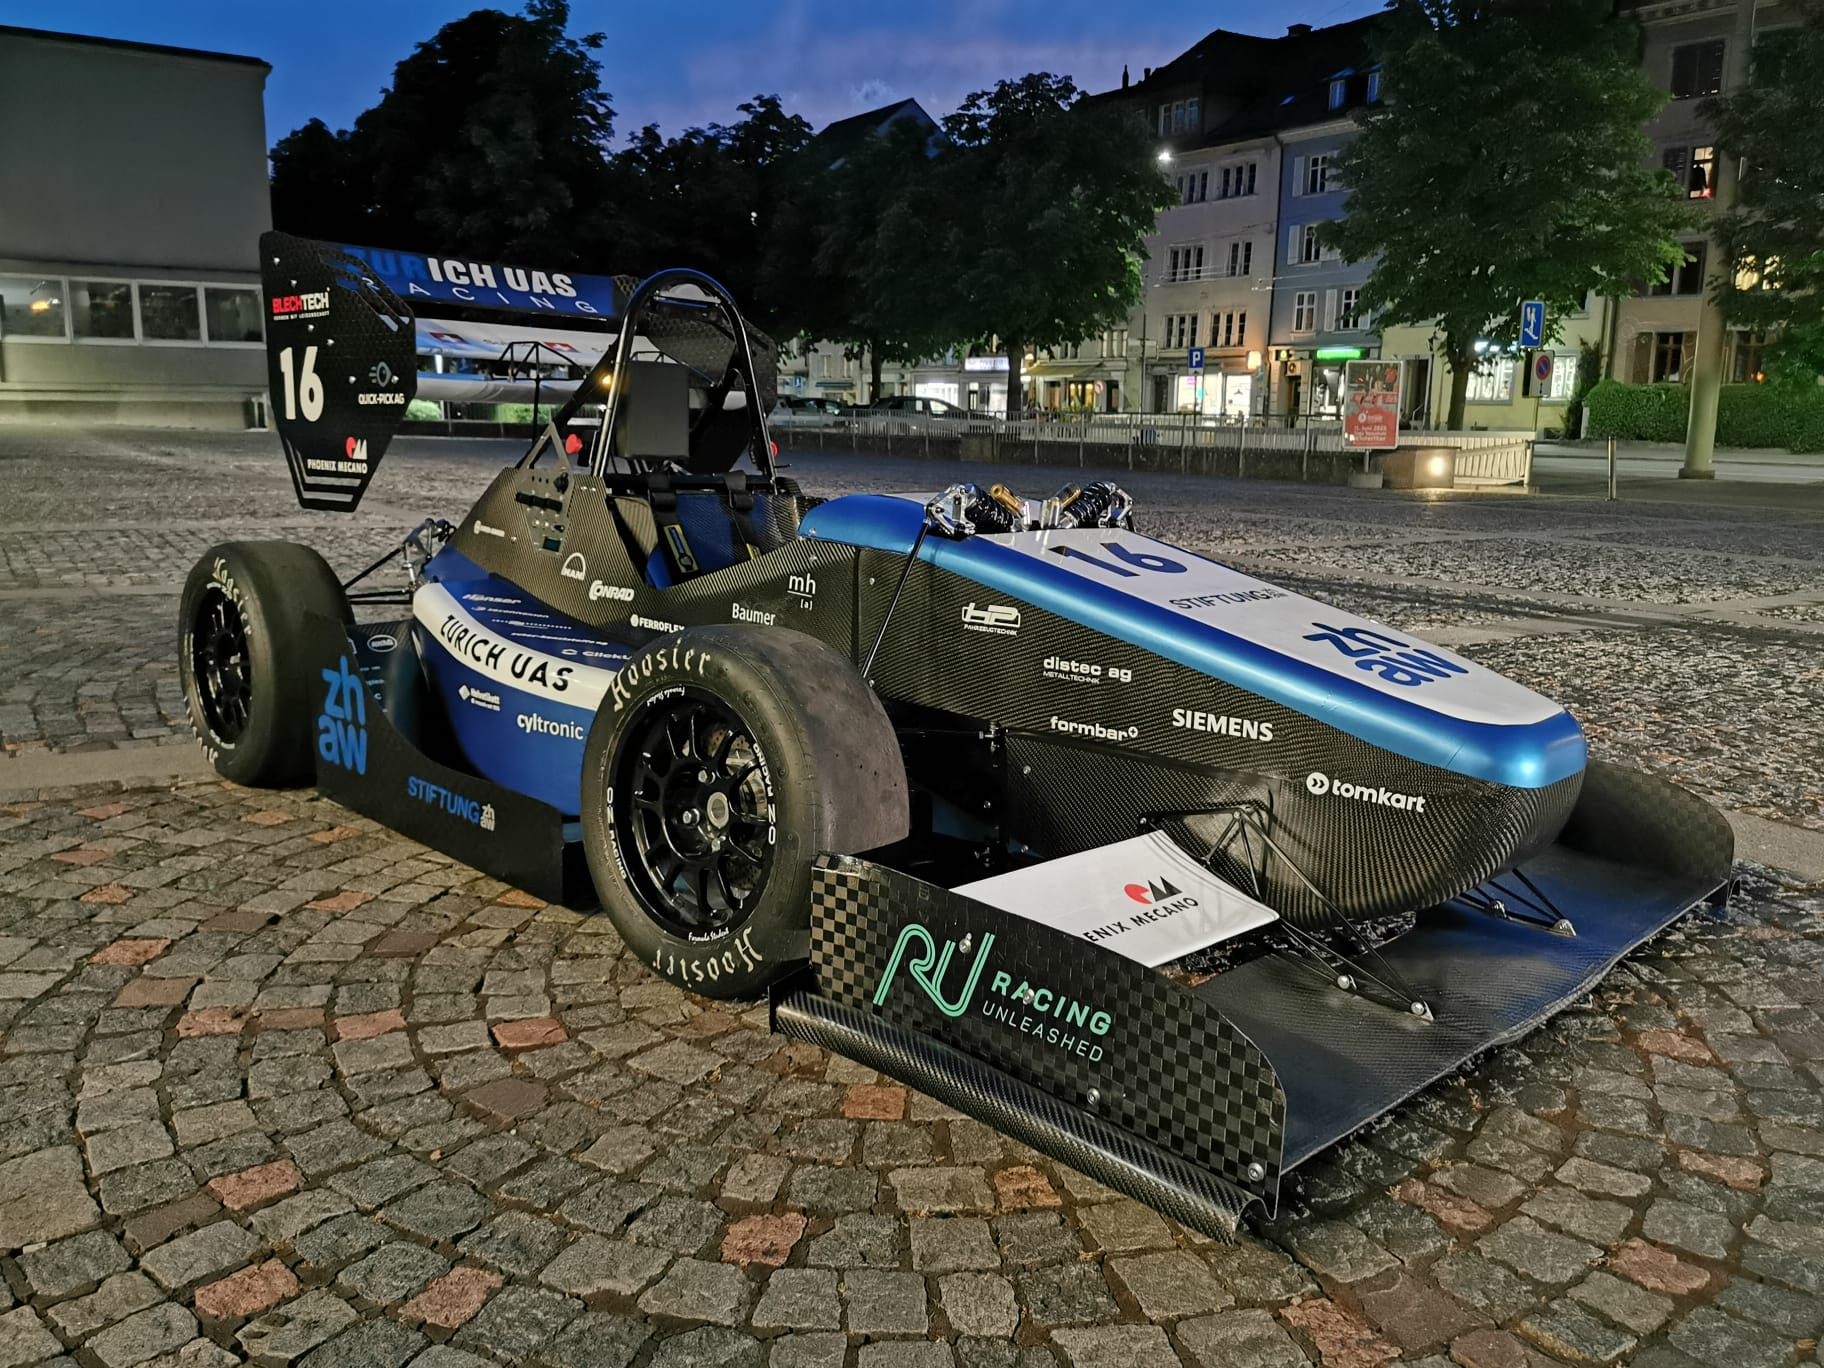
\includegraphics[width=12cm]{ZUR_Racecar_2.jpg}
    \caption{The new second race car of \acrlong{zur}.}
    \label{fig:ZUR Racecar 2}
\end{figure}

\section{Acceleration Track} \label{sec:Results Acceleration Track}
Acceleration:
Blue Cones: 14
Yellow Cones: 14
Orange Cones: 12
Big Orange Cones: 6
Exploration:
time of exploration cycle
0.0000s 0.0028s 0.0016s 43cycles 0.0671s
59 reference points

\begin{figure}[H]
    \centering
    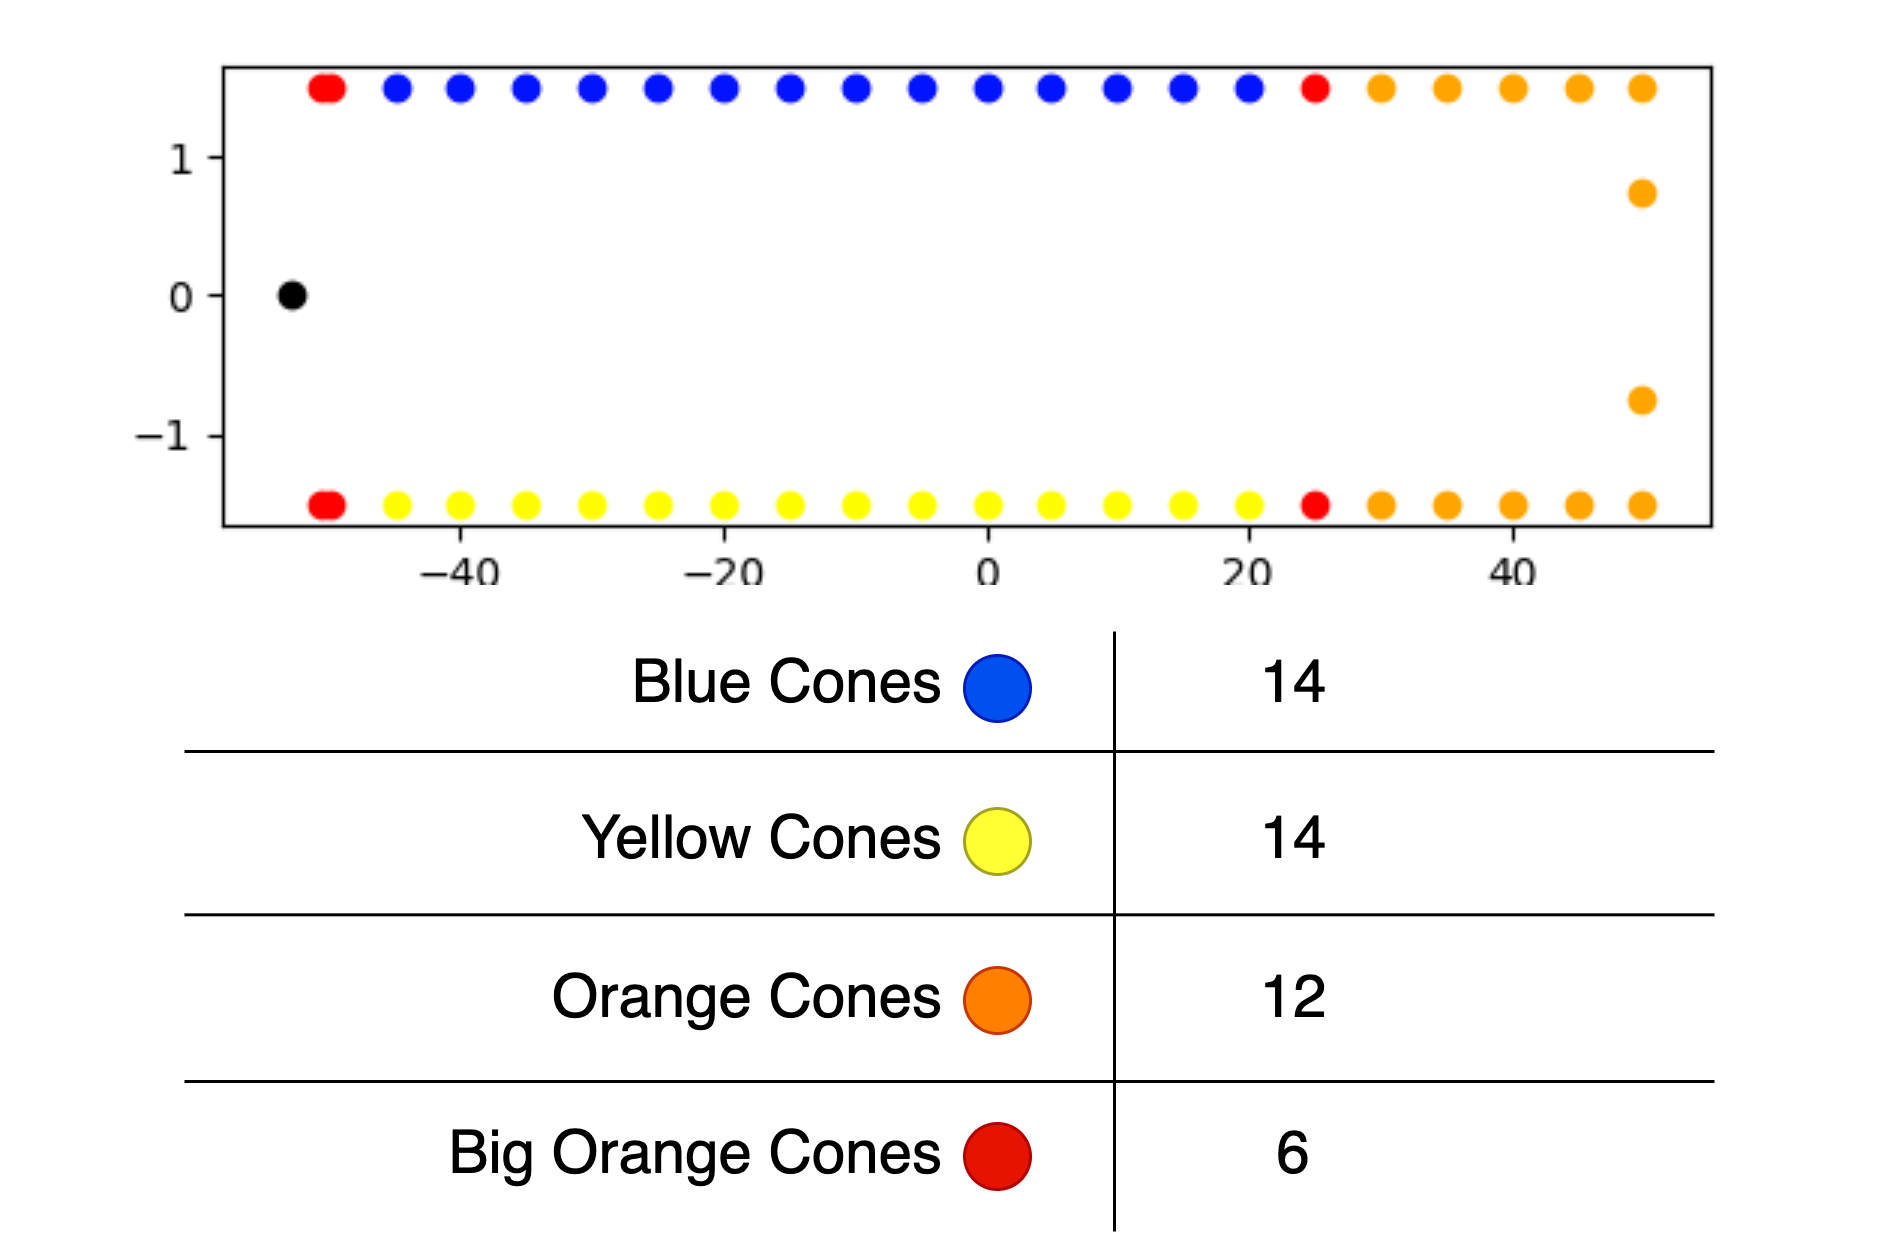
\includegraphics[width=\columnwidth]{Results_Acceleration_Initial.png}
    \caption{Overview of the Acceleration Track.}
    \label{fig:Results Acceleration Initial}
\end{figure}

Figure \ref{fig:Result Acceleration First Approaches} shows the first approach (a) and the second (b) approach side by side on the acceleration track, which was described in section \ref{sec:Dynamic Events}. The second approach calculated the middle points between the grouped four points used for the triangulation. In addition to the added points, a line was drawn to smoothen the track. Since the plot on (a) and (b) do not plot the start and the end cones (orange cones), they were just used as a basis for the final, more usable algorithm implementation seen in figure \ref{fig:Result Acceleration Final}.
\begin{figure}[H]
    \centering
    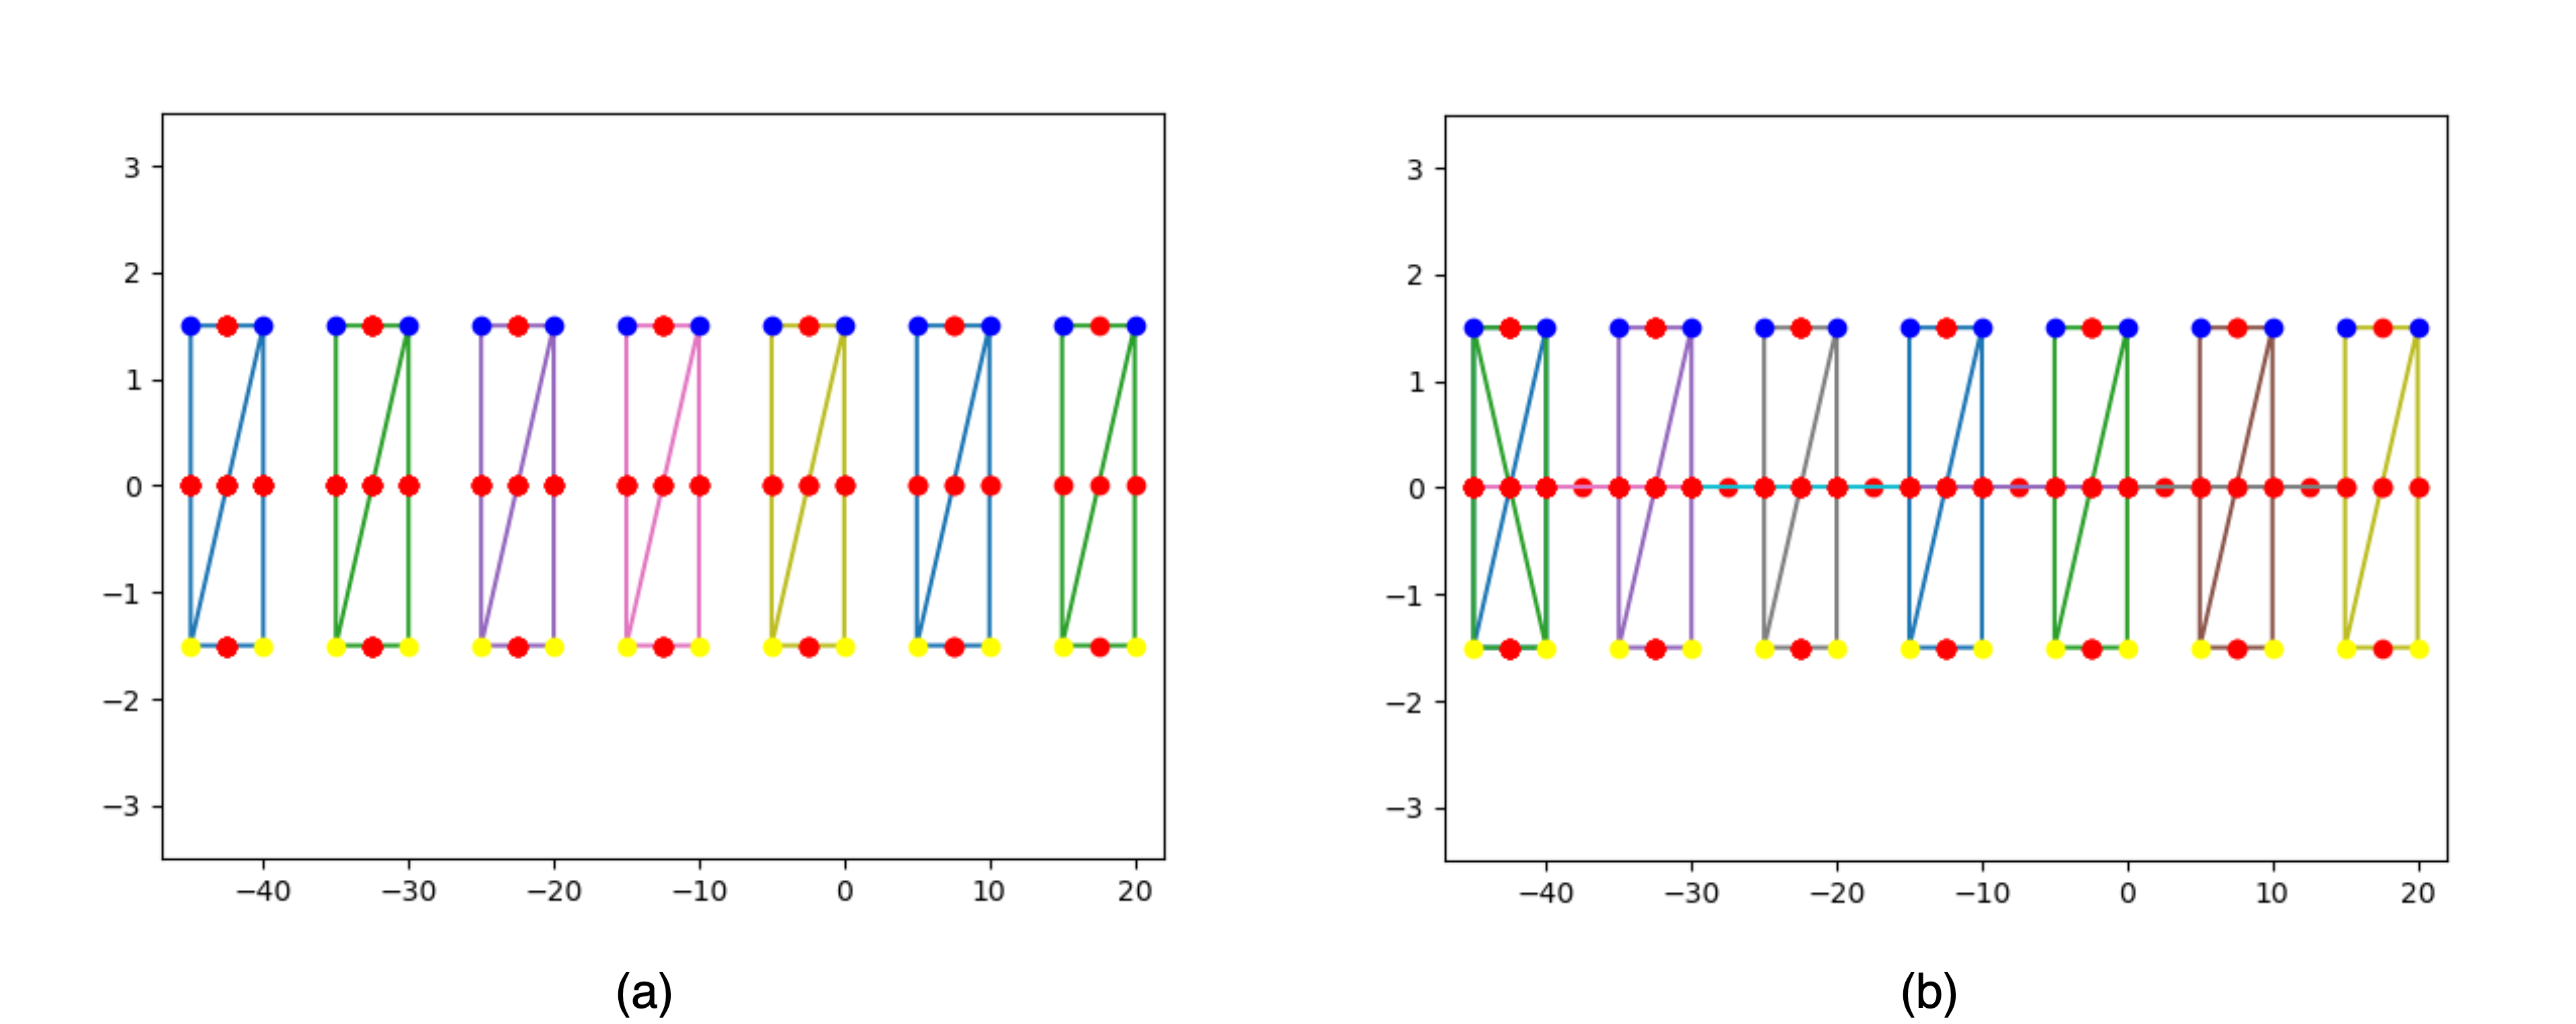
\includegraphics[width=\columnwidth]{Result_Acceleration_First_Approaches.png}
    \caption{Image (a) shows the first approach on the acceleration track, while image (b) shows the second while drawing a middle line.}
    \label{fig:Result Acceleration First Approaches}
\end{figure}
\begin{figure}[H]
    \centering
    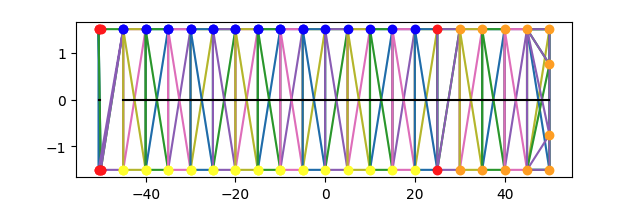
\includegraphics[width=\columnwidth]{Result_Acceleration_final.png}
    \caption{The image shows the final approach on the Acceleration track.}
    \label{fig:Result Acceleration Final}
\end{figure}

\section{Skidpad Track} \label{sec:Results Skidpad Track}
Skidpad:
Blue Cones: 30
Yellow Cones: 30
Orange Cones: 20
Big Orange Cones: 4
Exploration:
time of exploration cycle
0.0001s 0.0051s 0.0021s 103cycles 0.2169s
859 reference points

\begin{figure}[H]
    \centering
    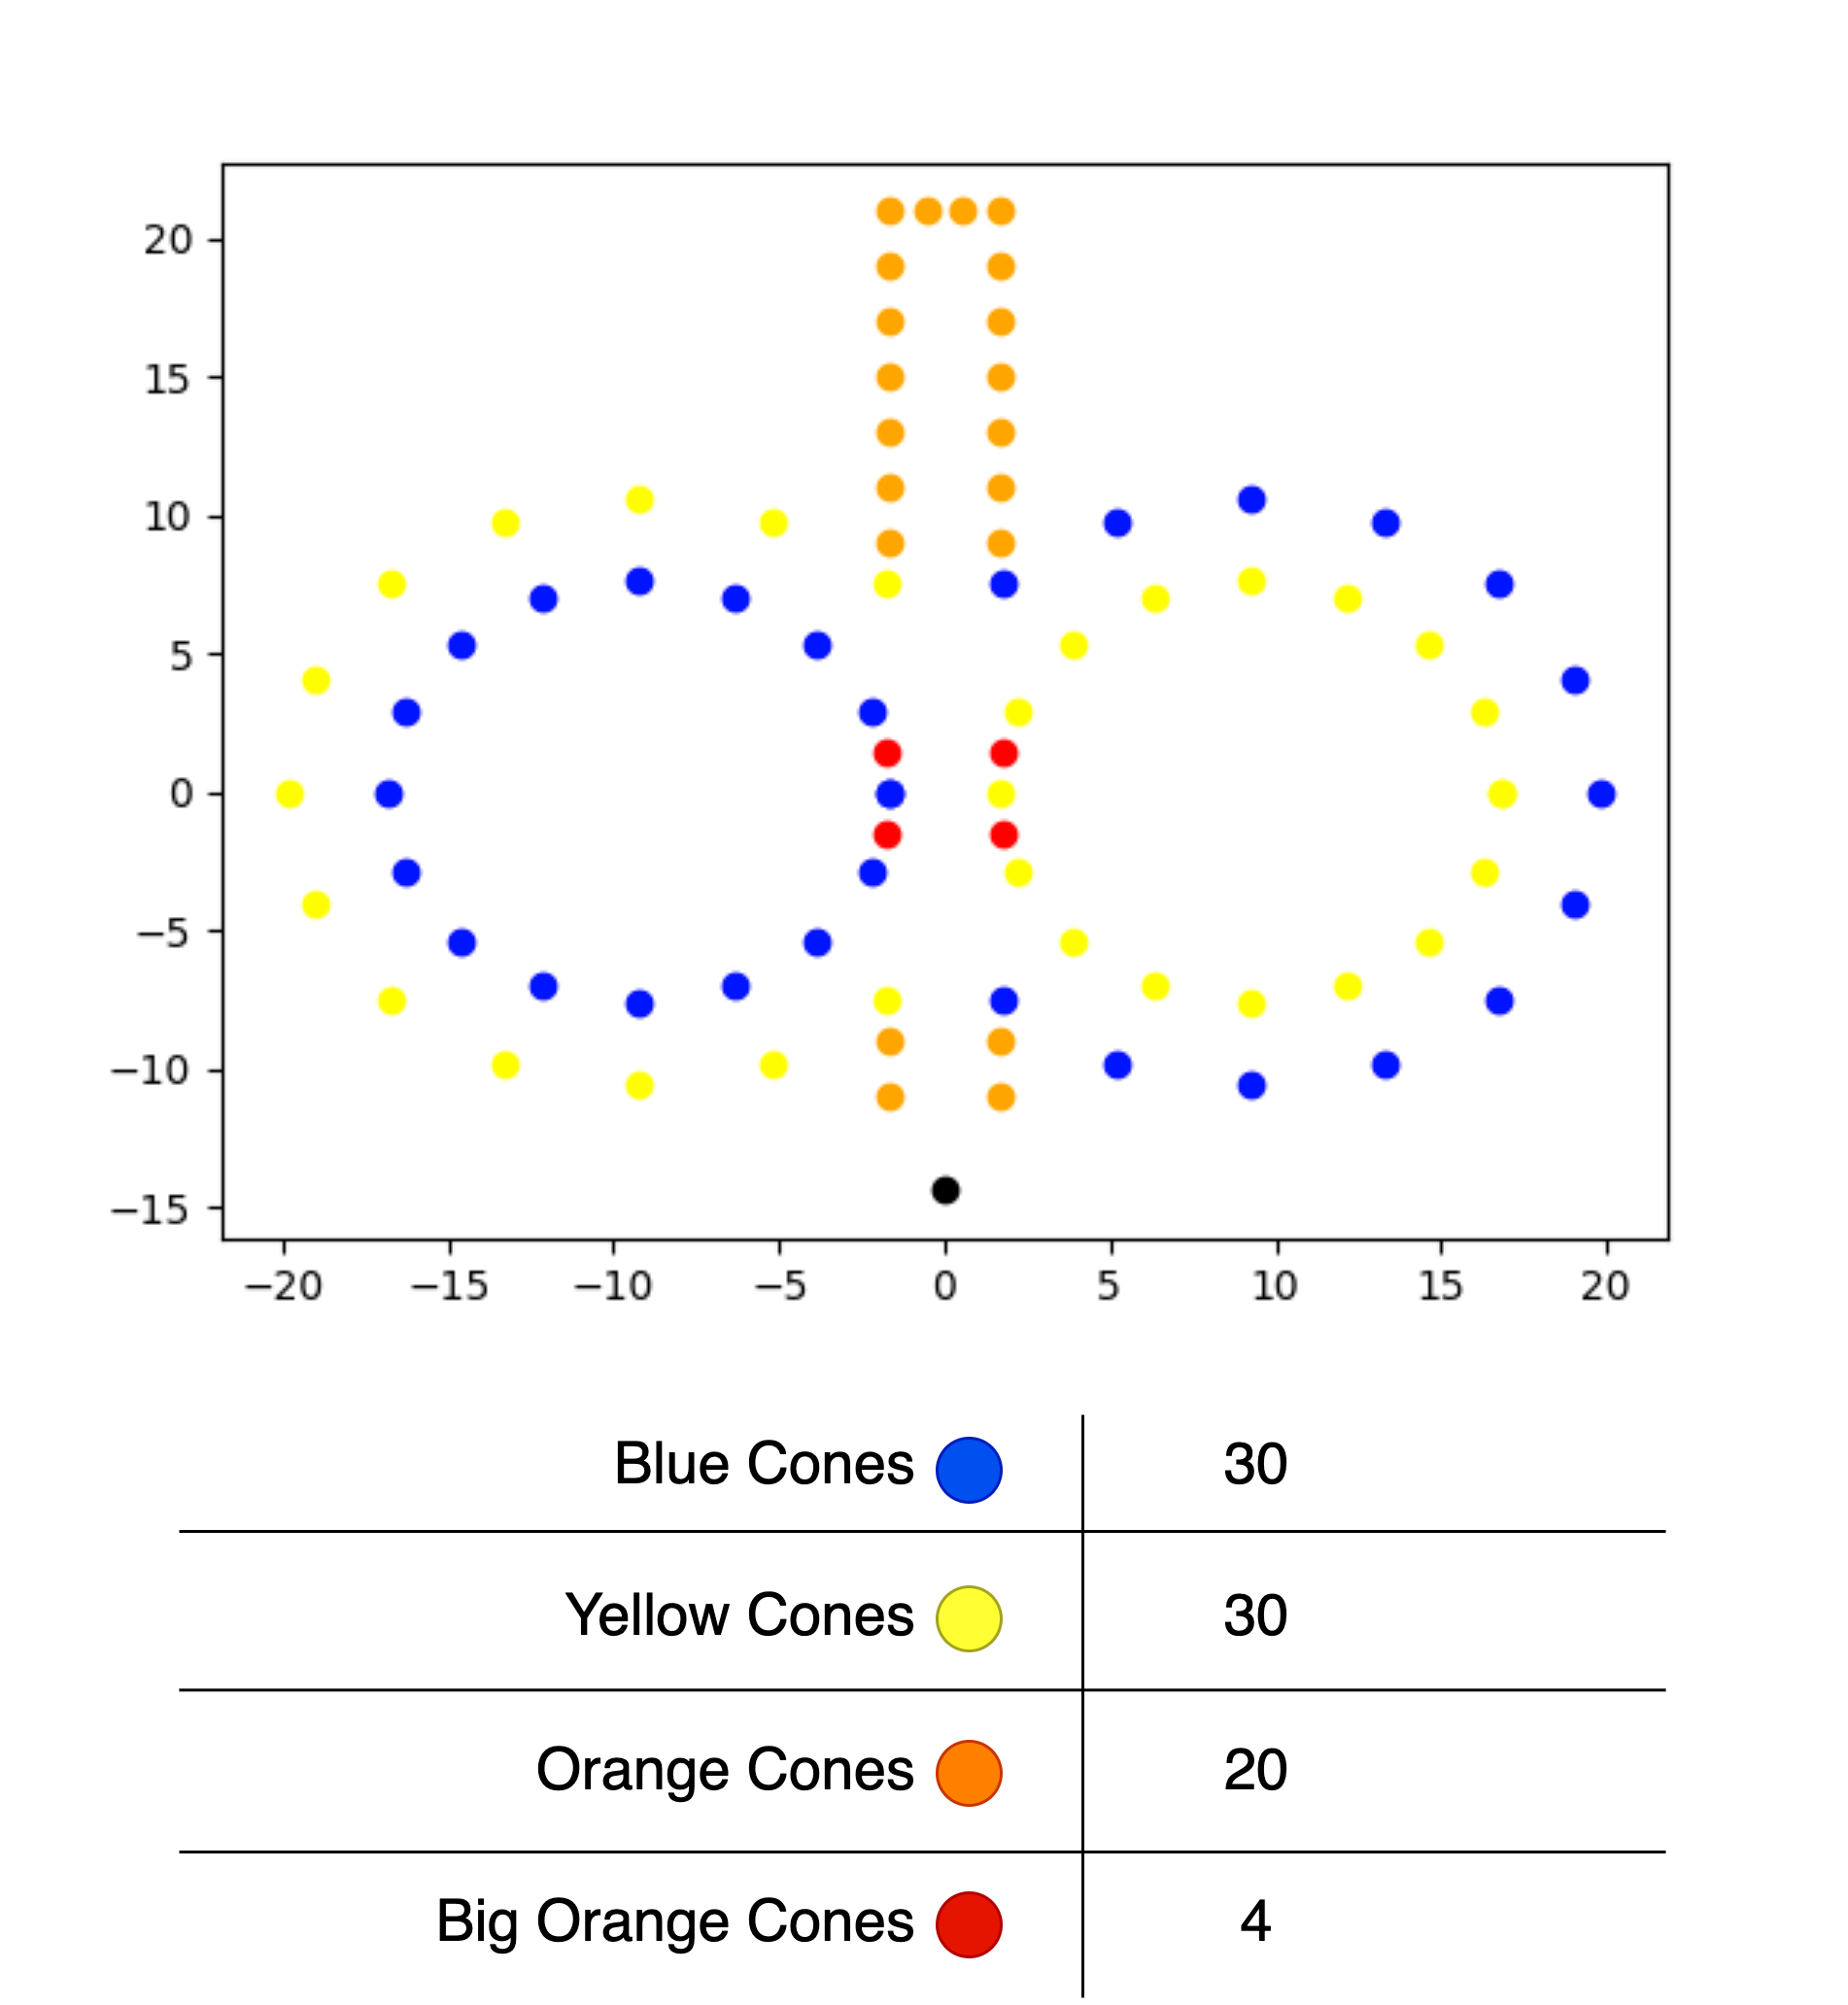
\includegraphics[width=\columnwidth]{Results_Skidpad_Initial.png}
    \caption{Overview of the Skidpad Track.}
    \label{fig:Results Skidpad Initial}
\end{figure}

The last example in figure \ref{fig:Result Skidpad Final} shows that the algorithm can also be applied on the ``Skidpad'' track.
\begin{figure}[H]
    \centering
    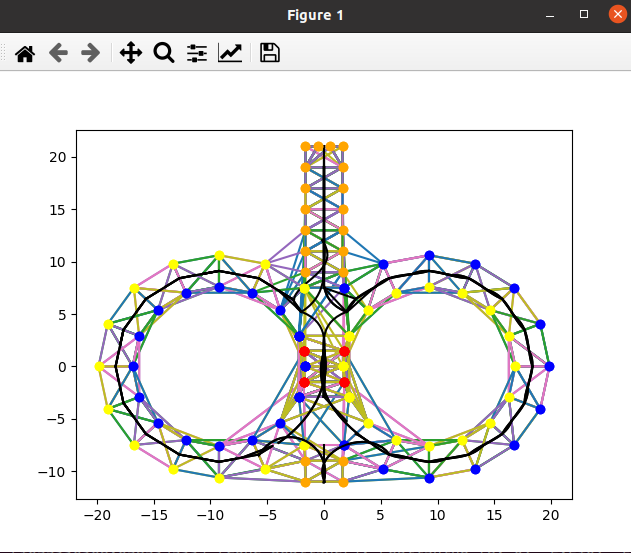
\includegraphics[width=\columnwidth]{Result_Skidpad_final.png}
    \caption{The calculation of the middle line with the Skidpad track.}
    \label{fig:Result Skidpad Final}
\end{figure}

\section{Small Track} \label{sec:Results Small Track}
Small Track:
Blue Cones: 37
Yellow Cones: 30
Orange Cones: 0
Big Orange Cones: 4
Exploration:
time of exploration cycle
0.0000s 0.0066s 0.0028s 71cycles 0.1974s
865 reference points
Optimization:
mincurv laps 1 2 3 5 8
reference points
Runtime 0.04s 0.08s 0.12s 0.22s 0.48s
lap time 9.17s 18.48s 28.24s 47.39s 78.44s
points 52 102 152 253 404
shortest 0.07s 20.60s 99p
iqp 0.10s 17.88s 102p

\begin{figure}[H]
    \centering
    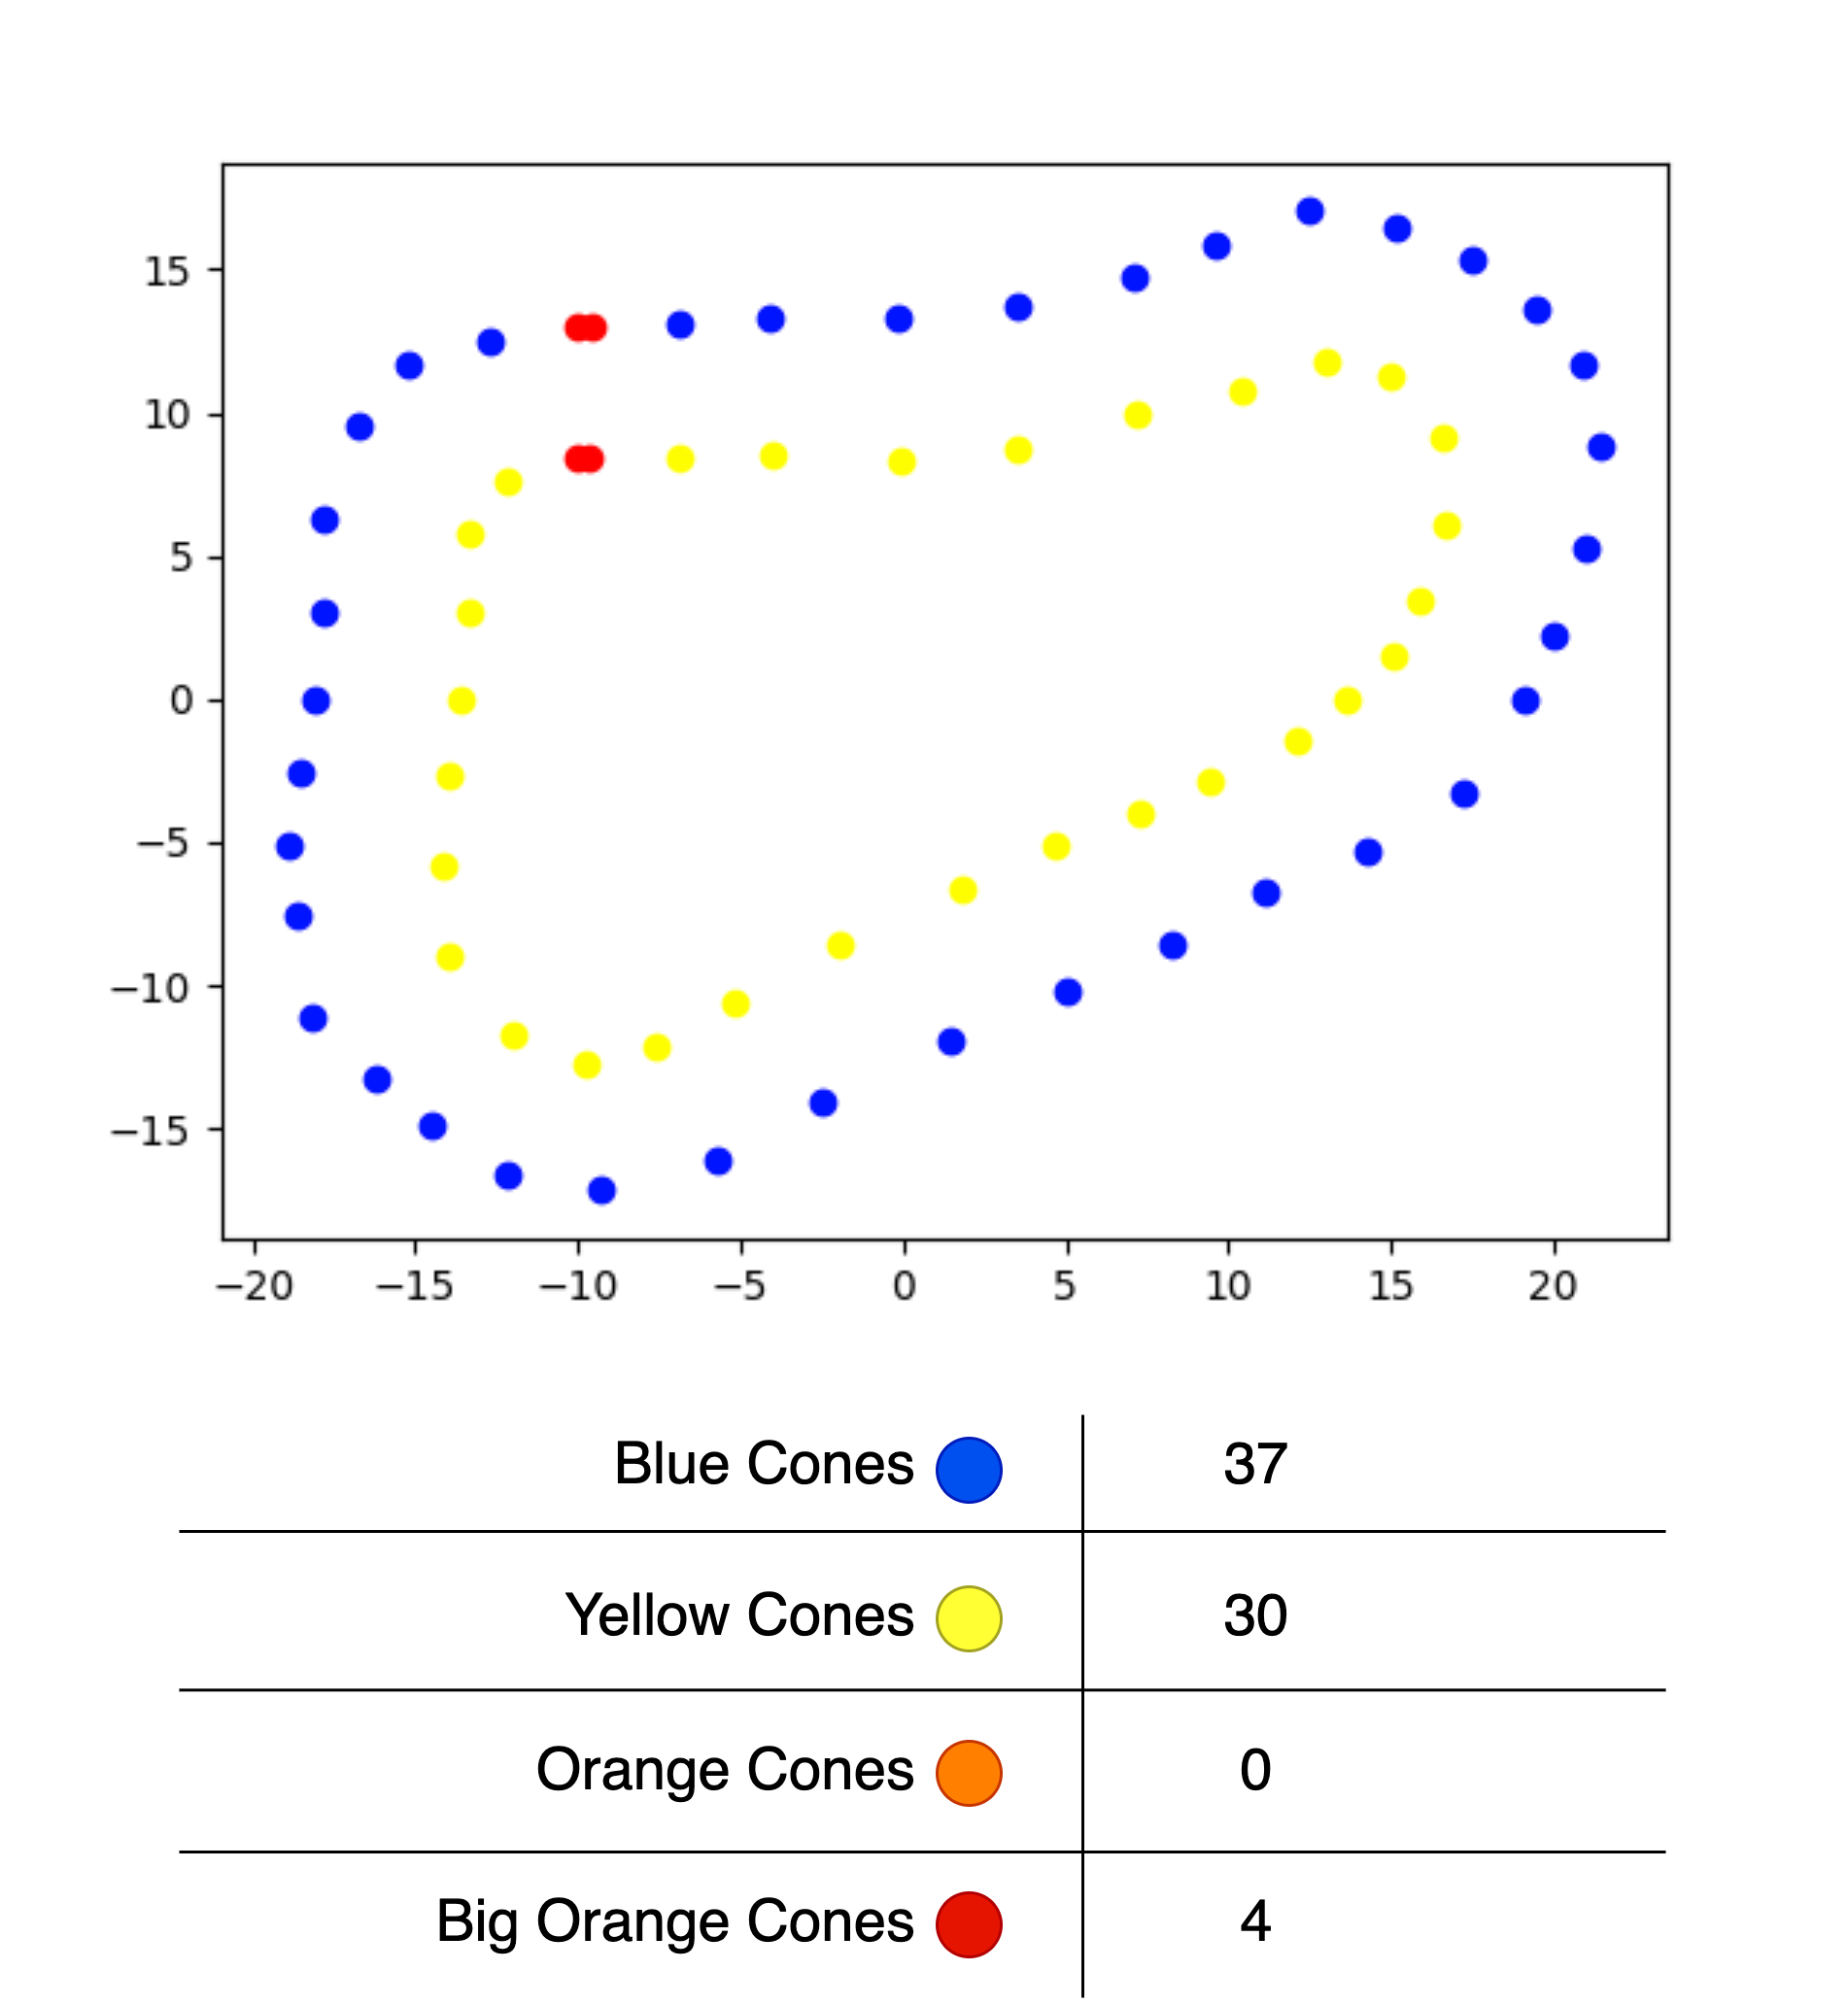
\includegraphics[width=\columnwidth]{Results_Small_Track_Initial.png}
    \caption{Overview of the Small Track.}
    \label{fig:Results Small Track Initial}
\end{figure}

\begin{figure}[H]
    \centering
    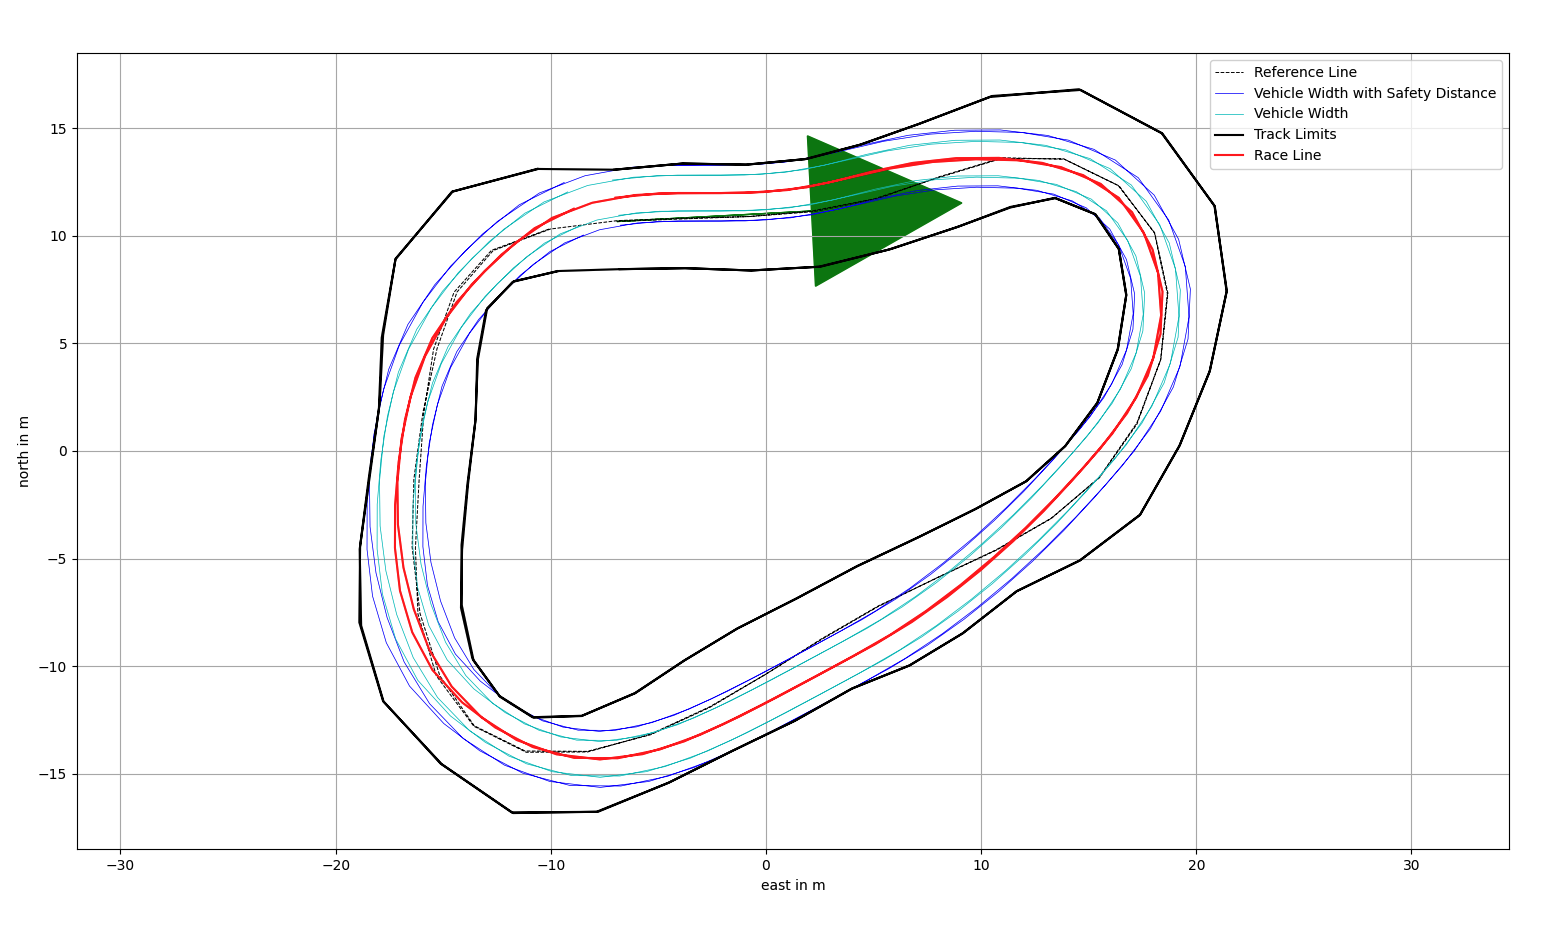
\includegraphics[width=\columnwidth]{Results_Optimization_Small_Track_Laps_2.png}
    \caption{Optimization on the Small Track for two laps.}
    \label{fig:Results Small Track Laps 2}
\end{figure}

The second track that was used for comparison is one of the \acrlong{tum} team, which is called ``Small Track''. \cite{tumftm_optimization_algoritm} This track helped to get an understanding of how the algorithm works on corners with fewer cones on the inner side than on the outer side. Figure \ref{fig:Result Small Track First Approaches} shows a progression of the improvements of the first implementation of the algorithm (a) to the second improved version (b) and the final version of the algorithm in figure \ref{fig:Result Small Track Final}. Again for the first and the second approach, the implementation of publishing the start and end cones (orange cones) was not made already.
\begin{figure}[H]
    \centering
    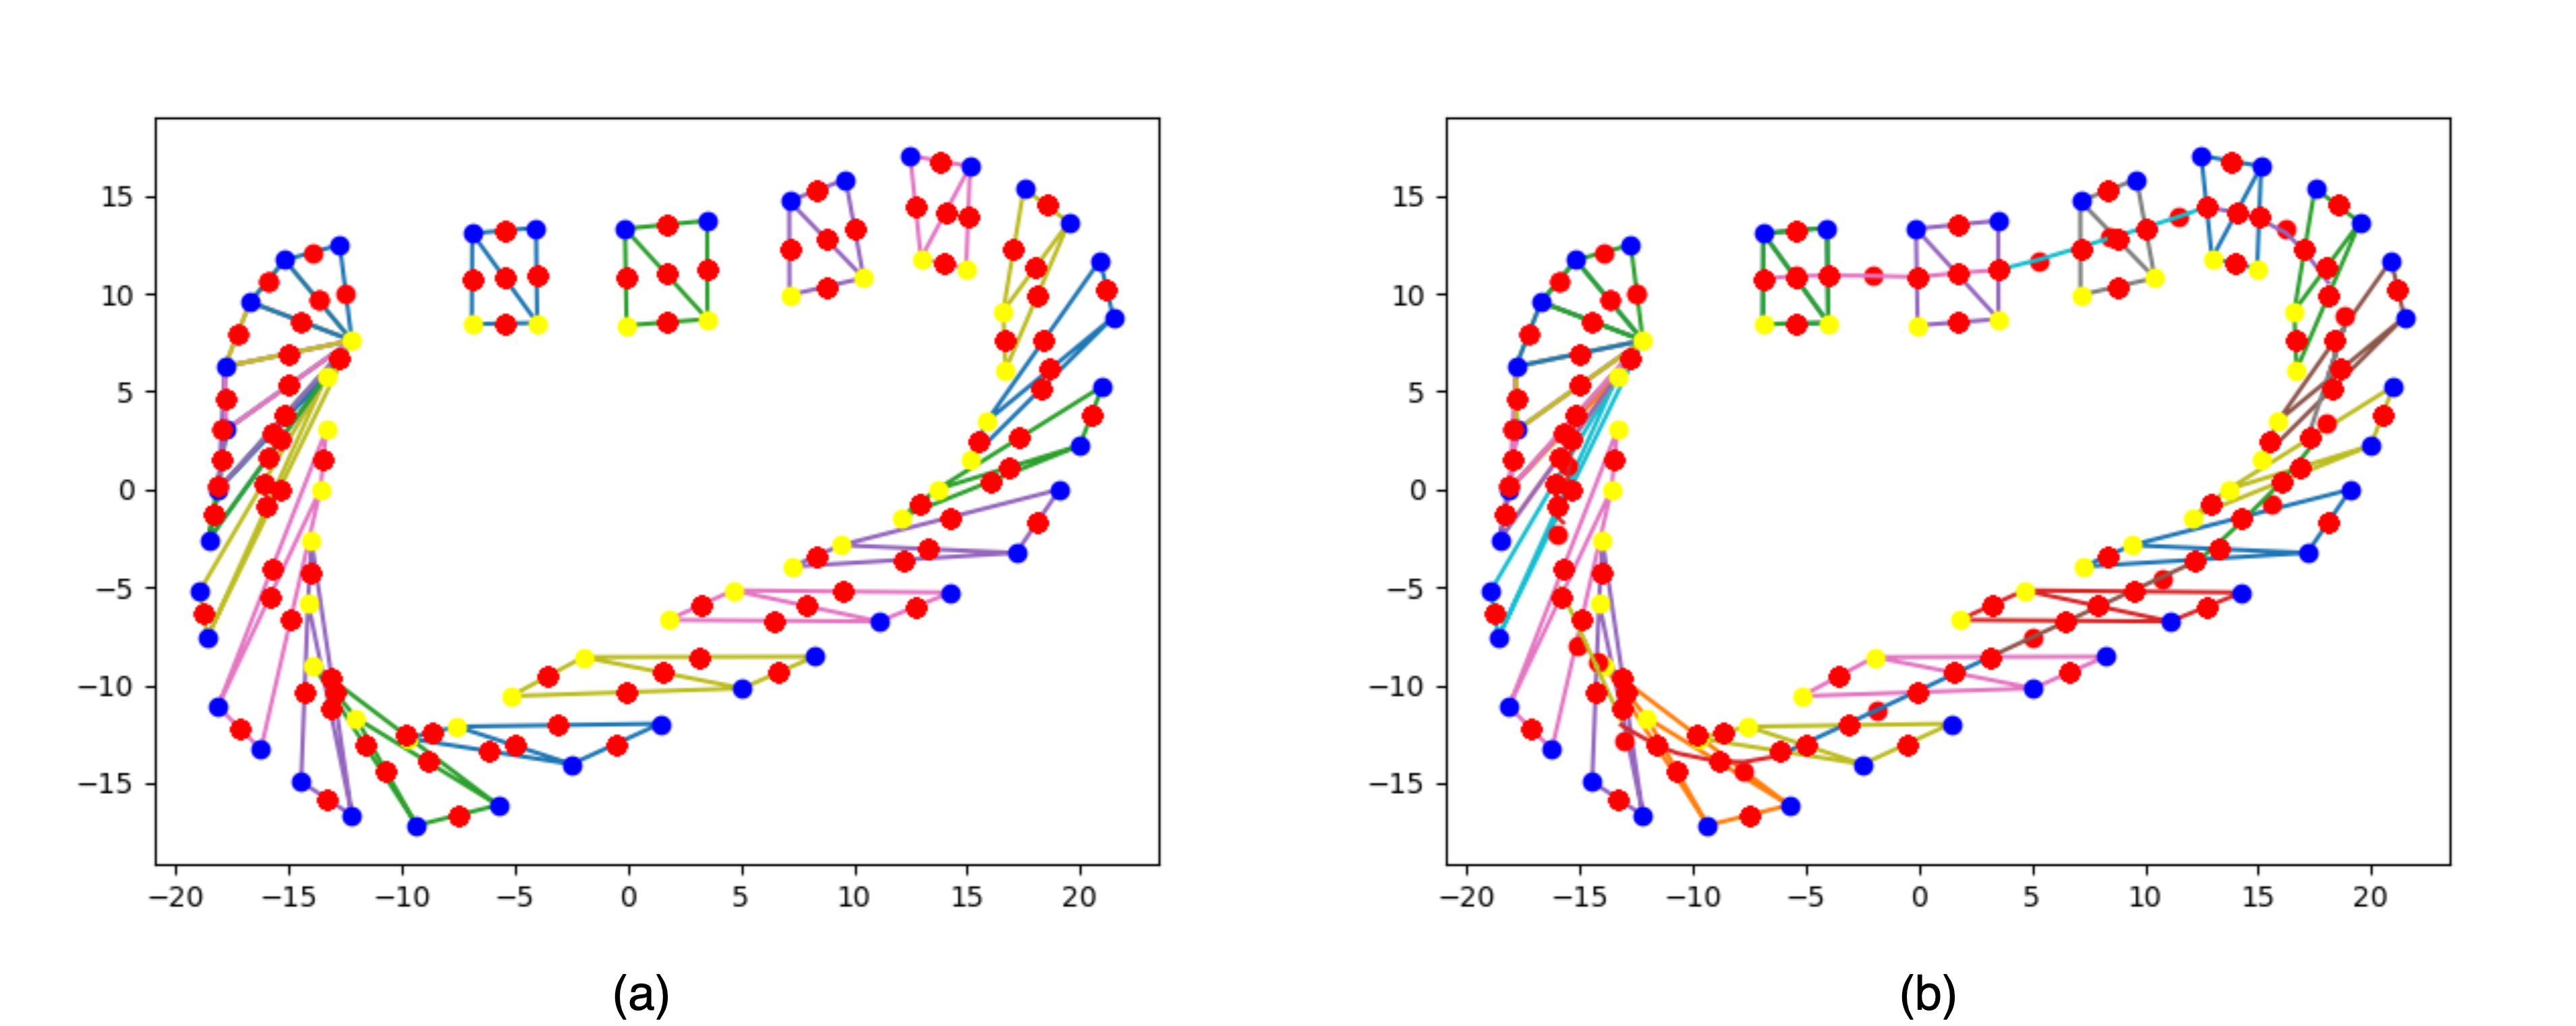
\includegraphics[width=\columnwidth]{Result_SmallTrack_First_Approaches.png}
    \caption{The progression of the improvements of the first implementation (a) to the second implementation (b) is shown.}
    \label{fig:Result Small Track First Approaches}
\end{figure}
\begin{figure}[H]
    \centering
    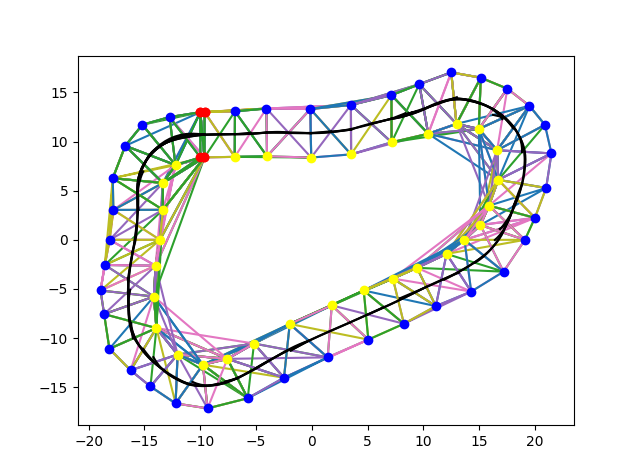
\includegraphics[width=\columnwidth]{Result_SmallTrack_final.png}
    \caption{The image shows the final approach on the Small Track.}
    \label{fig:Result Small Track Final}
\end{figure}

\section{Rand Track} \label{sec:Results Rand Track}
Rand:
Blue Cones: 99
Yellow Cones: 109
Orange Cones: 0
Big Orange Cones: 4
Exploration:
time of exploration cycle
0.0000s 0.0072s 0.0031s 215cycles 0.6730s
2635 reference points
Optimization:
mincurv laps 1 2 3 5 8
reference points
Runtime 0.12s 0.37s 0.92s 3.41s 13.18s
lap time 24.76s 49.83s 75.69s 129.65s 219.83s
points 194 388 581 967 1546
shortest 0.28s 60.84s 376p
iqp 0.82s 47.80s 384p

\begin{figure}[H]
    \centering
    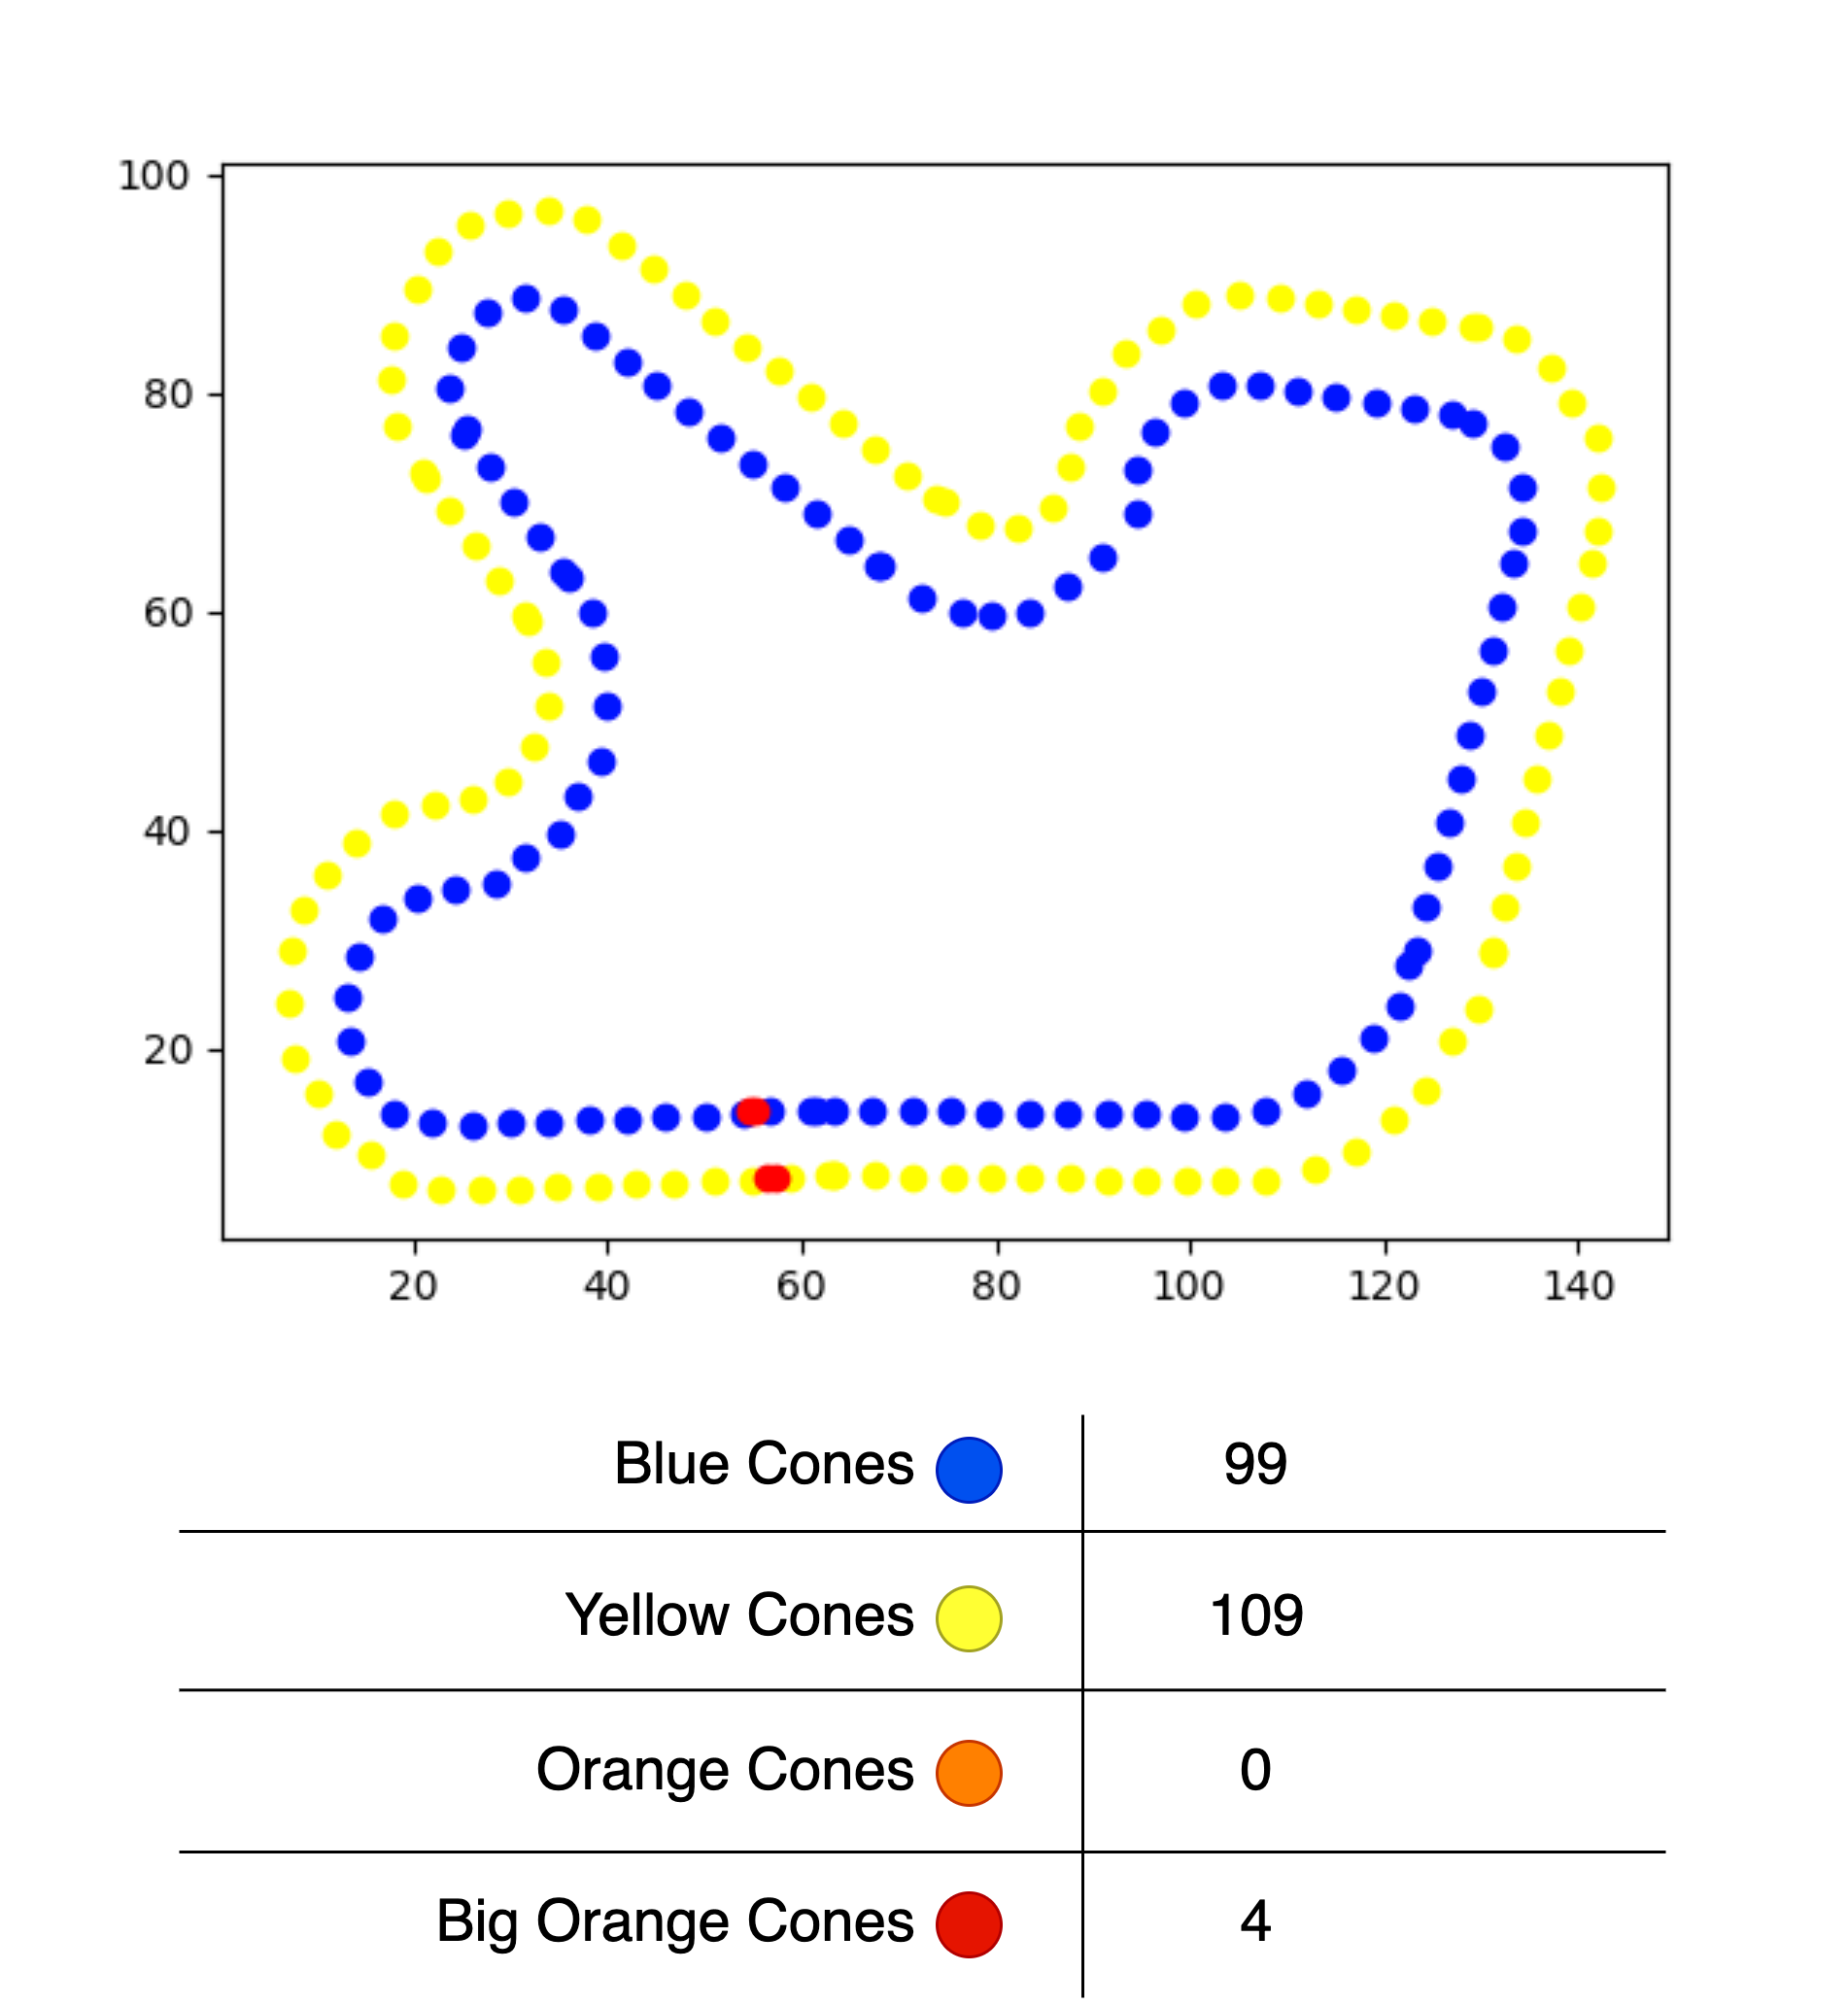
\includegraphics[width=\columnwidth]{Results_Rand_Initial.png}
    \caption{Overview of the Rand Track.}
    \label{fig:Results Rand Initial}
\end{figure}

\begin{figure}[H]
    \centering
    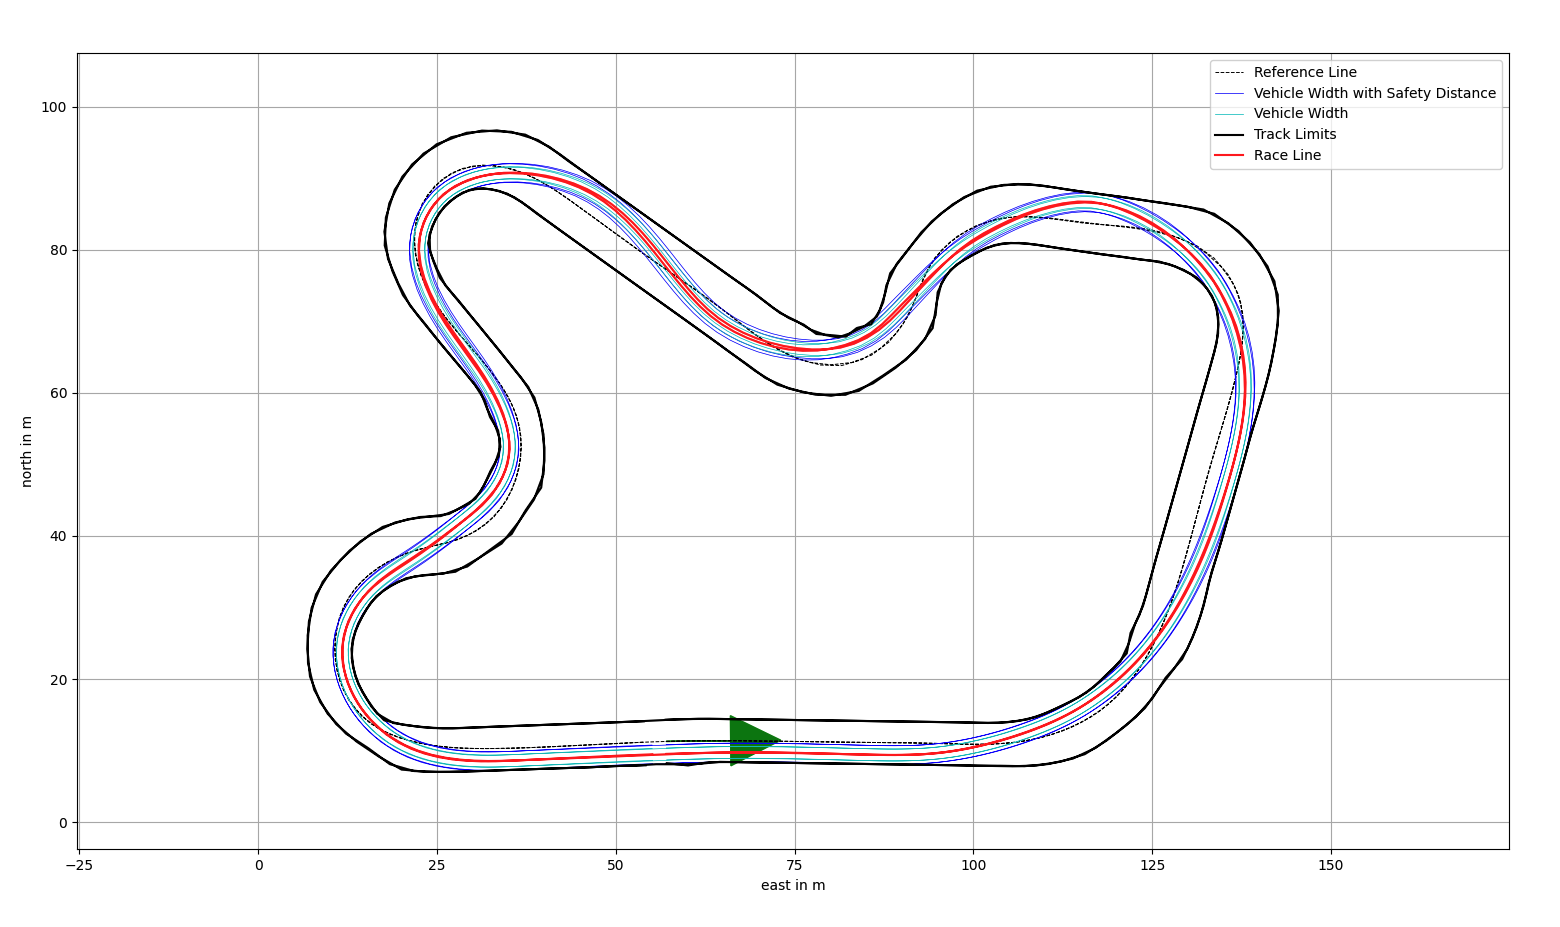
\includegraphics[width=\columnwidth]{Results_Optimization_Rand_Laps_2.png}
    \caption{Optimization on the Rand Track for two laps.}
    \label{fig:Results Rand Laps 2}
\end{figure}

The next track, which is shown in figure \ref{fig:Result Rand Final} that was used for testing the final implementation, was the ``Rand'' track. It has more cones and curvature than the ``Small Track'' and shows an example of a track that could have been used for the Track Drive event in the competition, as described in section \ref{sec:Dynamic Events}.
\begin{figure}[H]
    \centering
    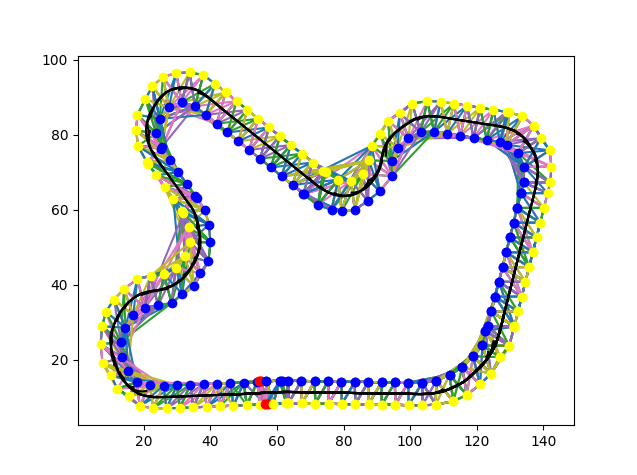
\includegraphics[width=\columnwidth]{Result_Rand_final.png}
    \caption{The ``Rand'' track with the final algorithm implementation.}
    \label{fig:Result Rand Final}
\end{figure}

\section{Competition 2021 Track} \label{sec:Results Competition 2021 Track}
Comp 2021:
Blue Cones: 156
Yellow Cones: 156
Orange Cones: 0
Big Orange Cones: 4
Exploration:
time of exploration cycle
0.0000s 0.0069s 0.0021s 320cycles 0.6621s
3425 reference points
Optimization:
mincurv laps 1 2 3 5 8
reference points
Runtime 0.12s 0.30s 0.57s 1.66s 5.37s
lap time 29.37s 58.87s 90.06s 146.97s 234.88s
points 130 259 386 642 1029
shortest 0.25s 59.29s 248p
iqp DNF

\begin{figure}[H]
    \centering
    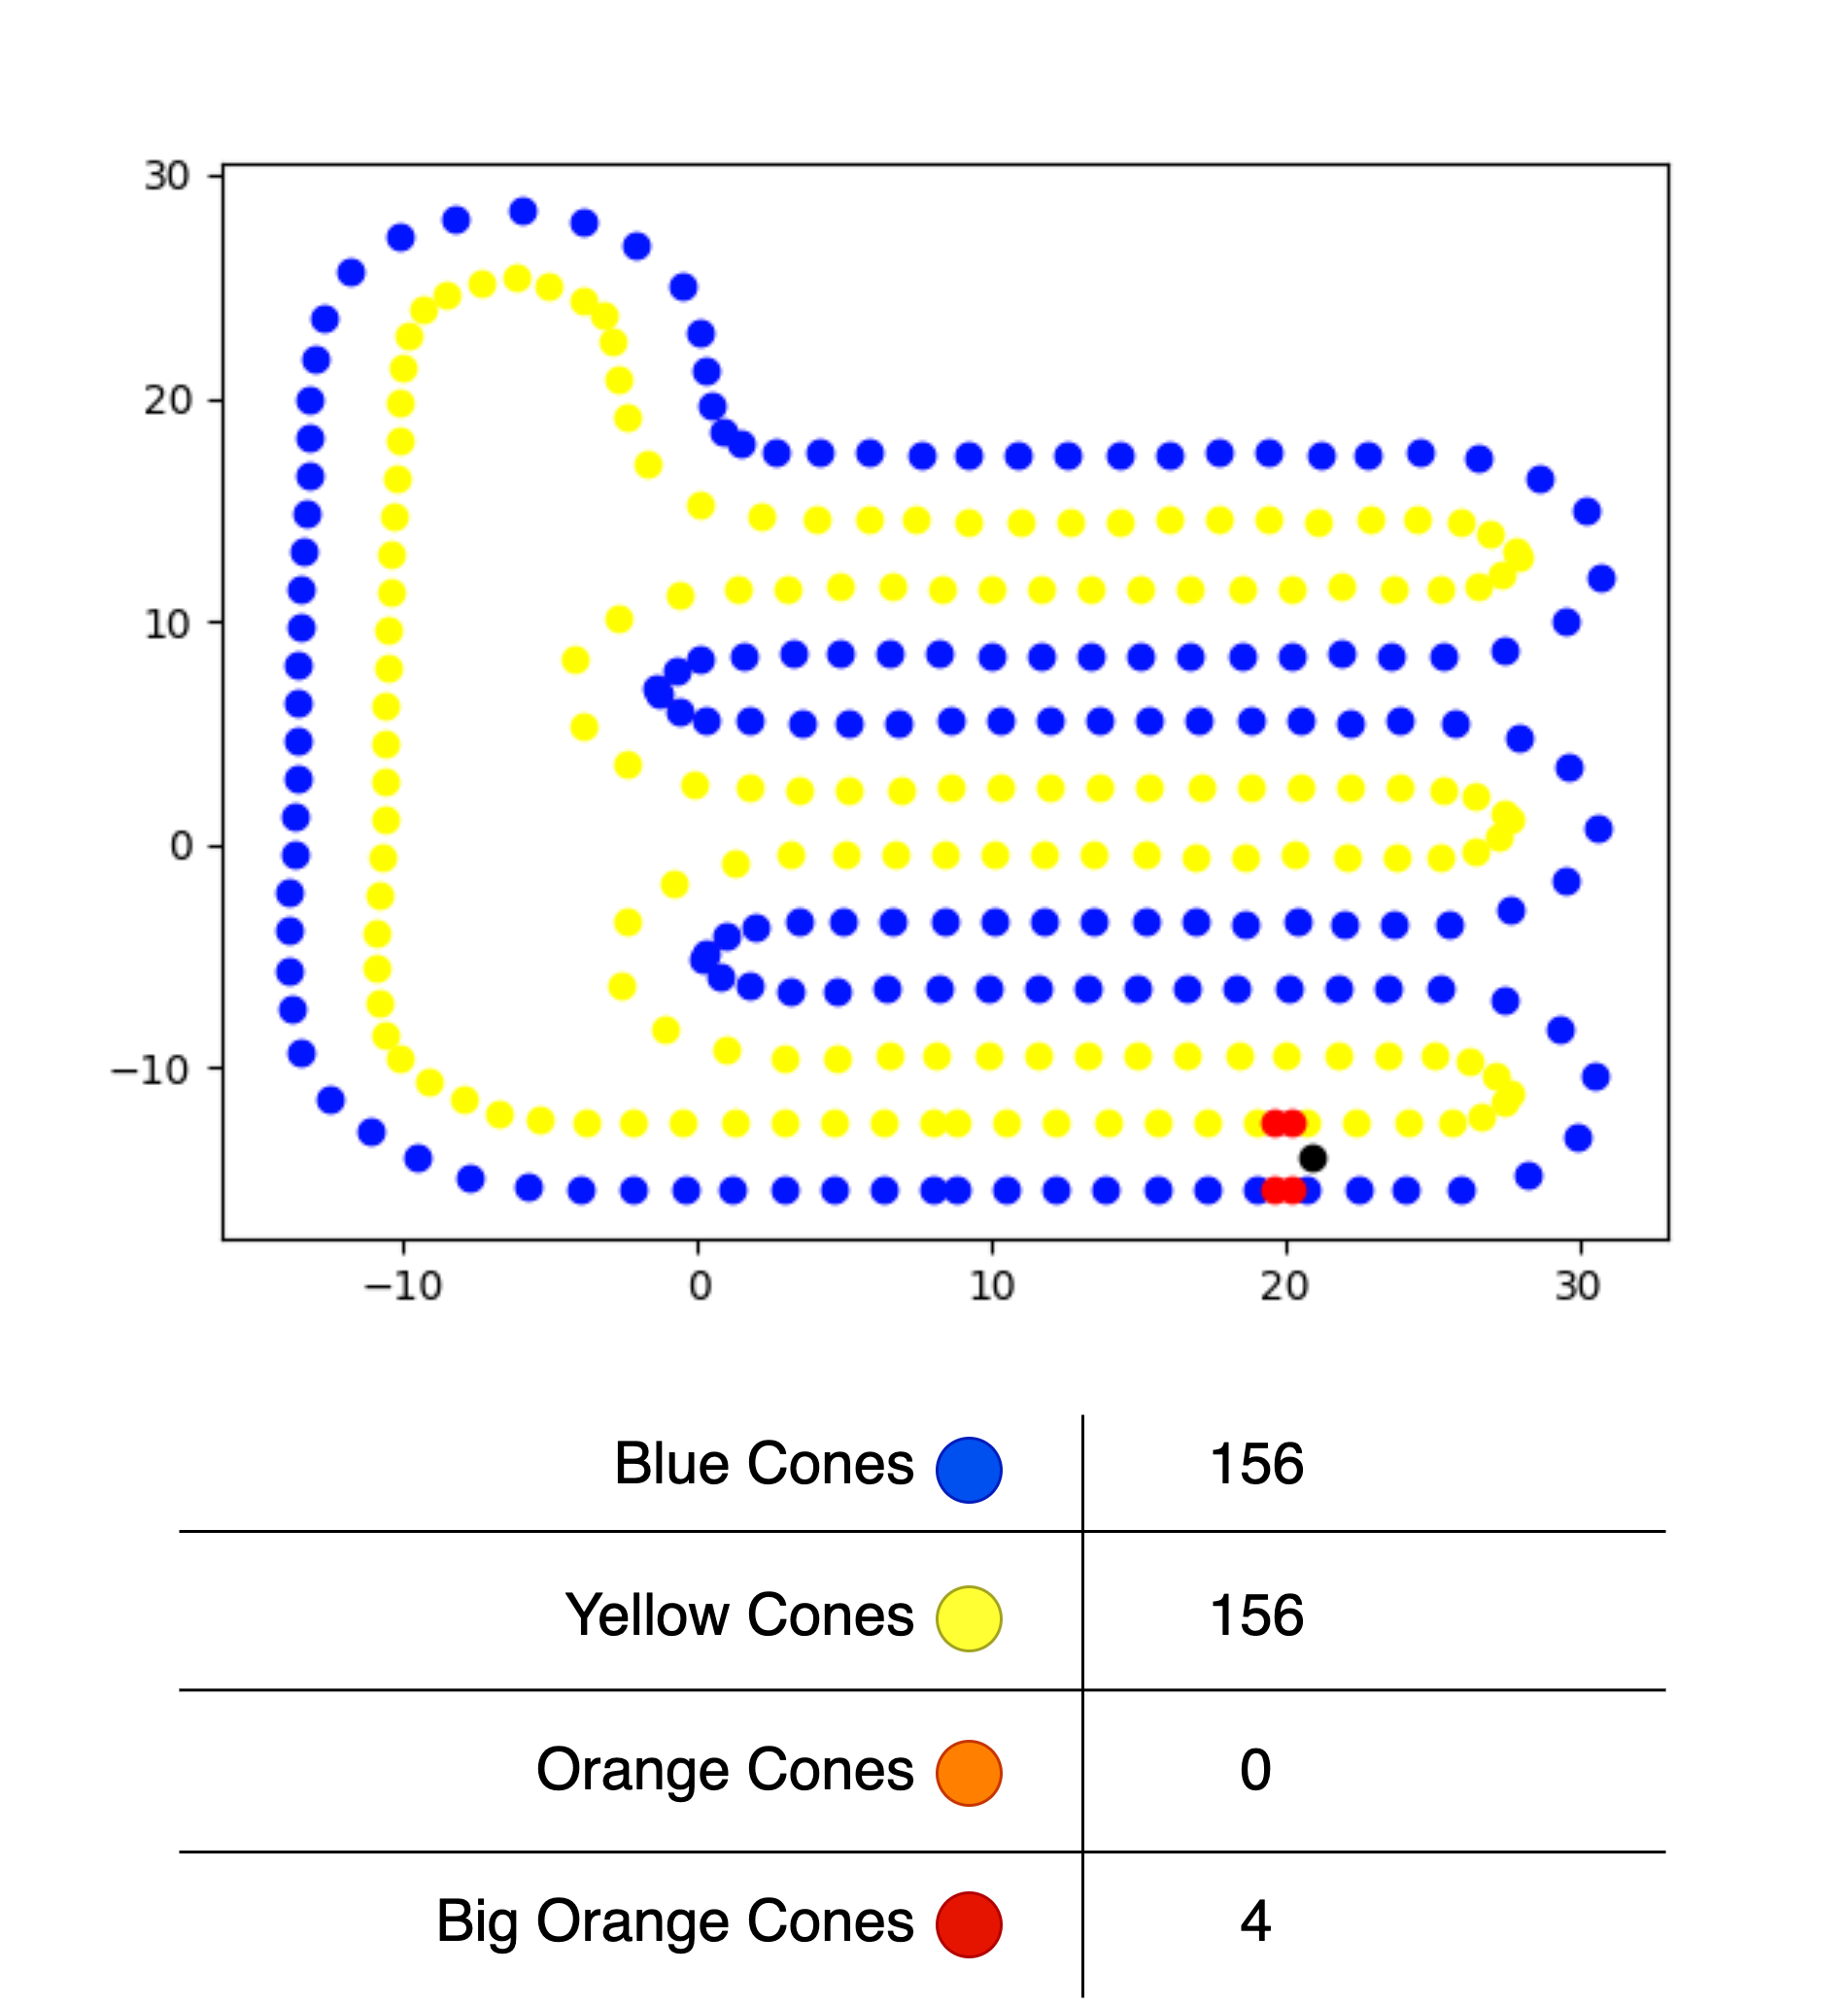
\includegraphics[width=\columnwidth]{Results_Comp_2021_Initial.png}
    \caption{Overview of the Competition 2021 Track.}
    \label{fig:Results Comp 2021 Initial}
\end{figure}

\begin{figure}[H]
    \centering
    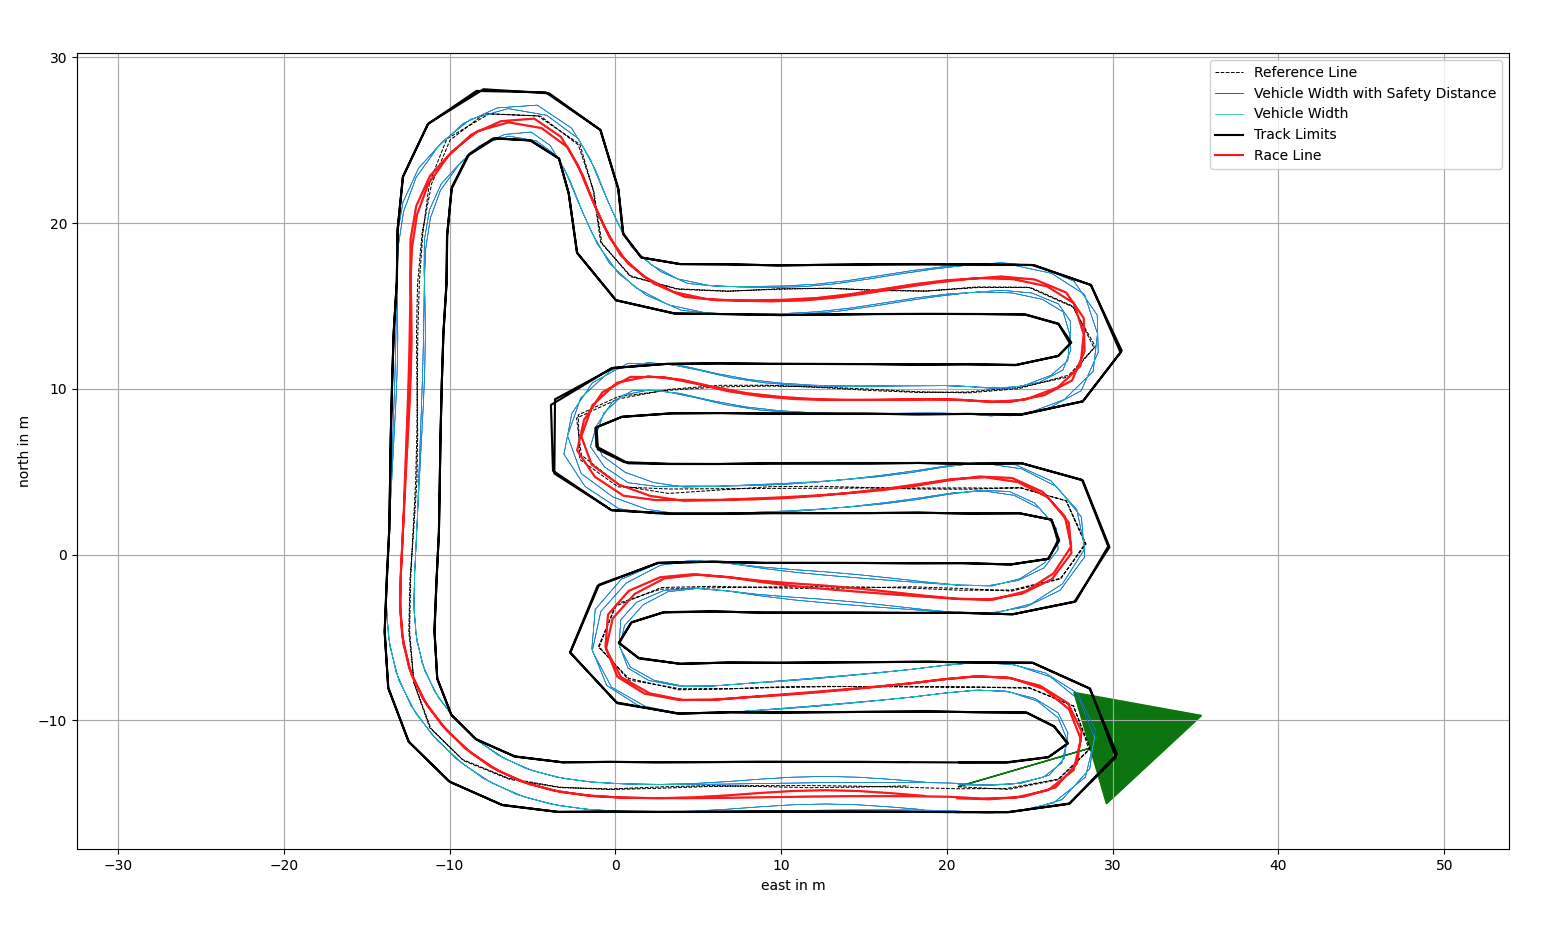
\includegraphics[width=\columnwidth]{Results_Optimization_Comp_2021_Laps_2.png}
    \caption{Optimization on the Competition 2021 Track for two laps.}
    \label{fig:Results Comp 2021 Laps 2}
\end{figure}

Furthermore, a track which was used for a competition in 2021 is shown in figure \ref{fig:Result Comp 2021 Final} with the applied final exploration algorithm. The track consists of more corners than the ``Rand'' track.
\begin{figure}[H]
    \centering
    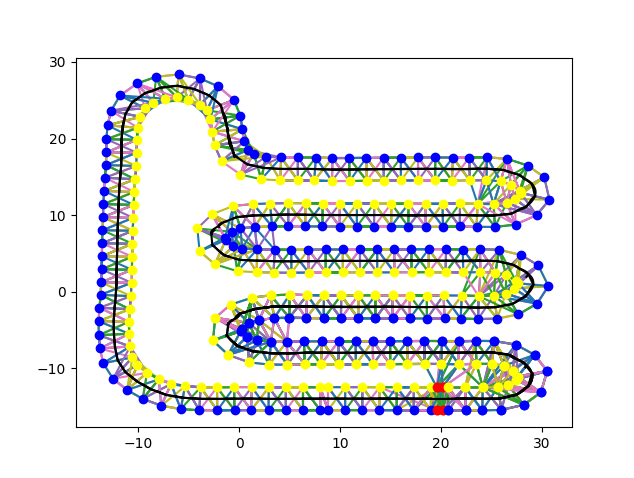
\includegraphics[width=\columnwidth]{Result_Comp2021_final.png}
    \caption{The result of the final exploration algorithm applied on the competition track of 2021.}
    \label{fig:Result Comp 2021 Final}
\end{figure}

\section{Garden Light Track} \label{sec:Results Garden Light Track}
Garden Light:
Blue Cones: 101
Yellow Cones: 99
Orange Cones: 0
Big Orange Cones: 4
Exploration:
time of exploration cycle
0.0000s 0.0076s 0.0029s 205cycles 0.5926s
2631 reference points
Optimization:
mincurv laps 1 2 3 5 8
reference points
Runtime 0.07s 0.17s 0.29s 0.74s 2.03s
lap time 25.20s 48.72s 71.59s 117.31s 190.31s
points 88 173 258 428 682
shortest 0.15s 47.39s 159p
iqp DNF

\begin{figure}[H]
    \centering
    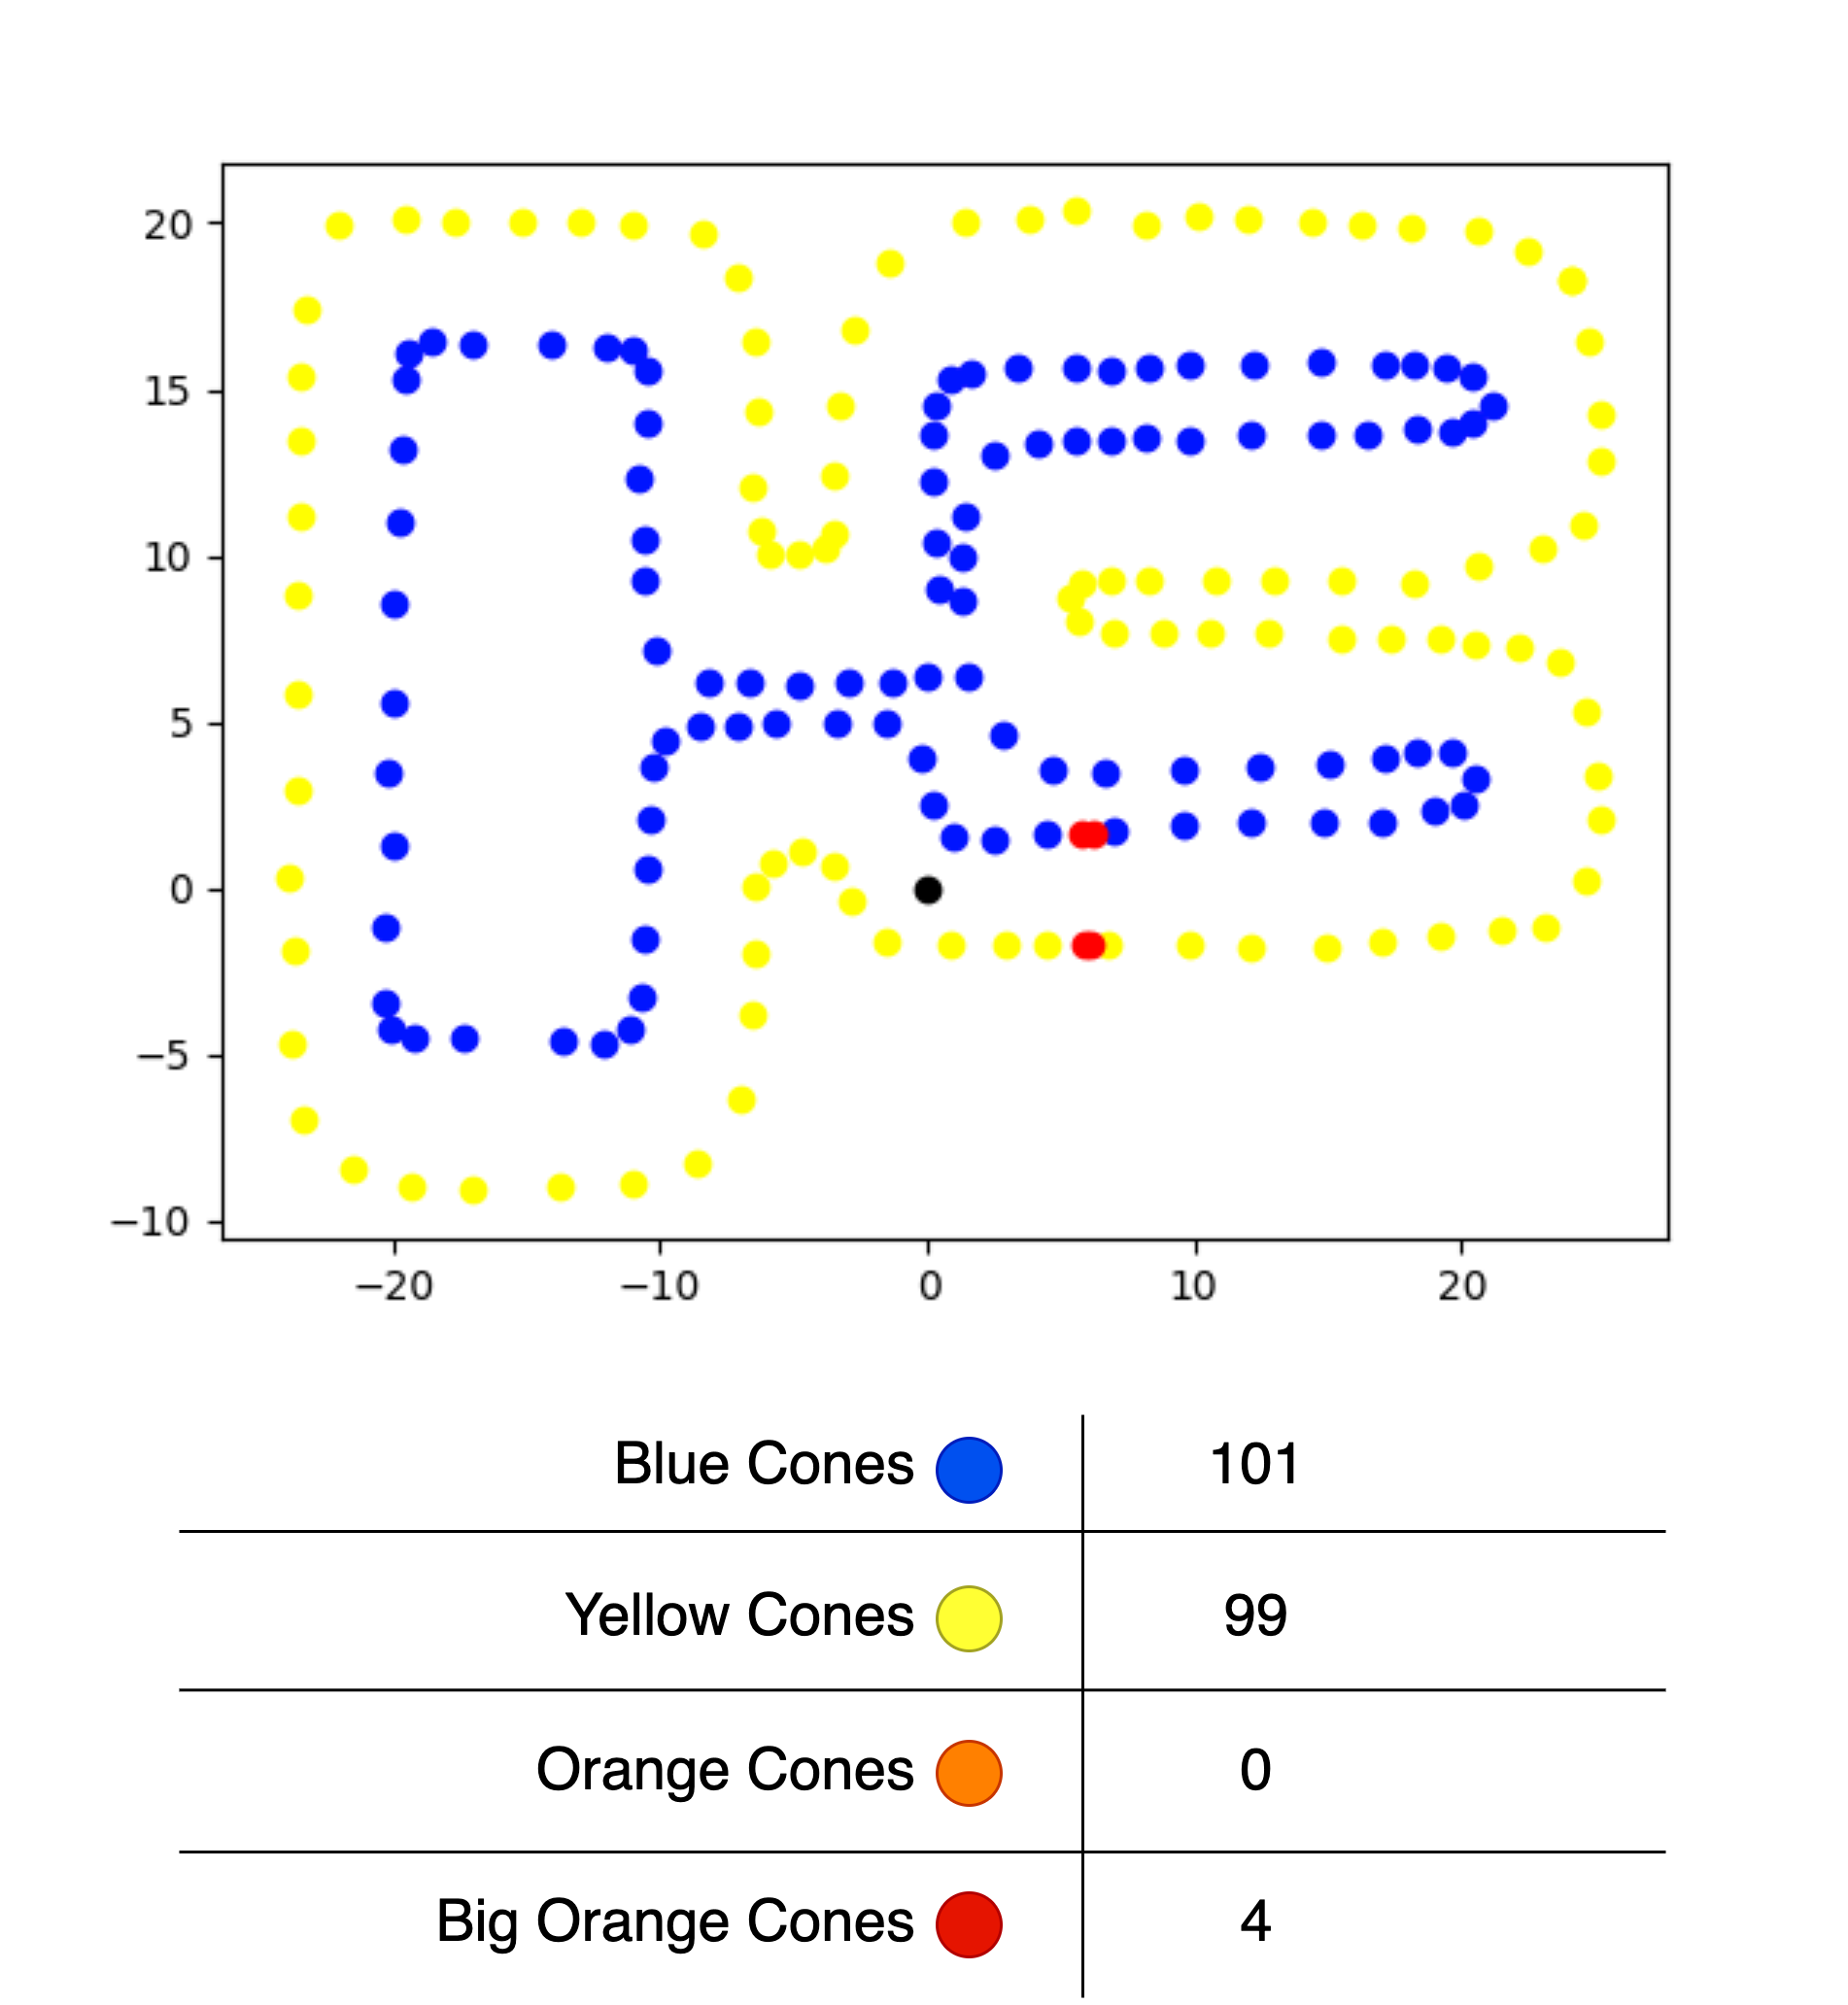
\includegraphics[width=\columnwidth]{Results_Garden_Light_Initial.png}
    \caption{Overview of the Garden Light Track.}
    \label{fig:Results Garden Light Initial}
\end{figure}

\begin{figure}[H]
    \centering
    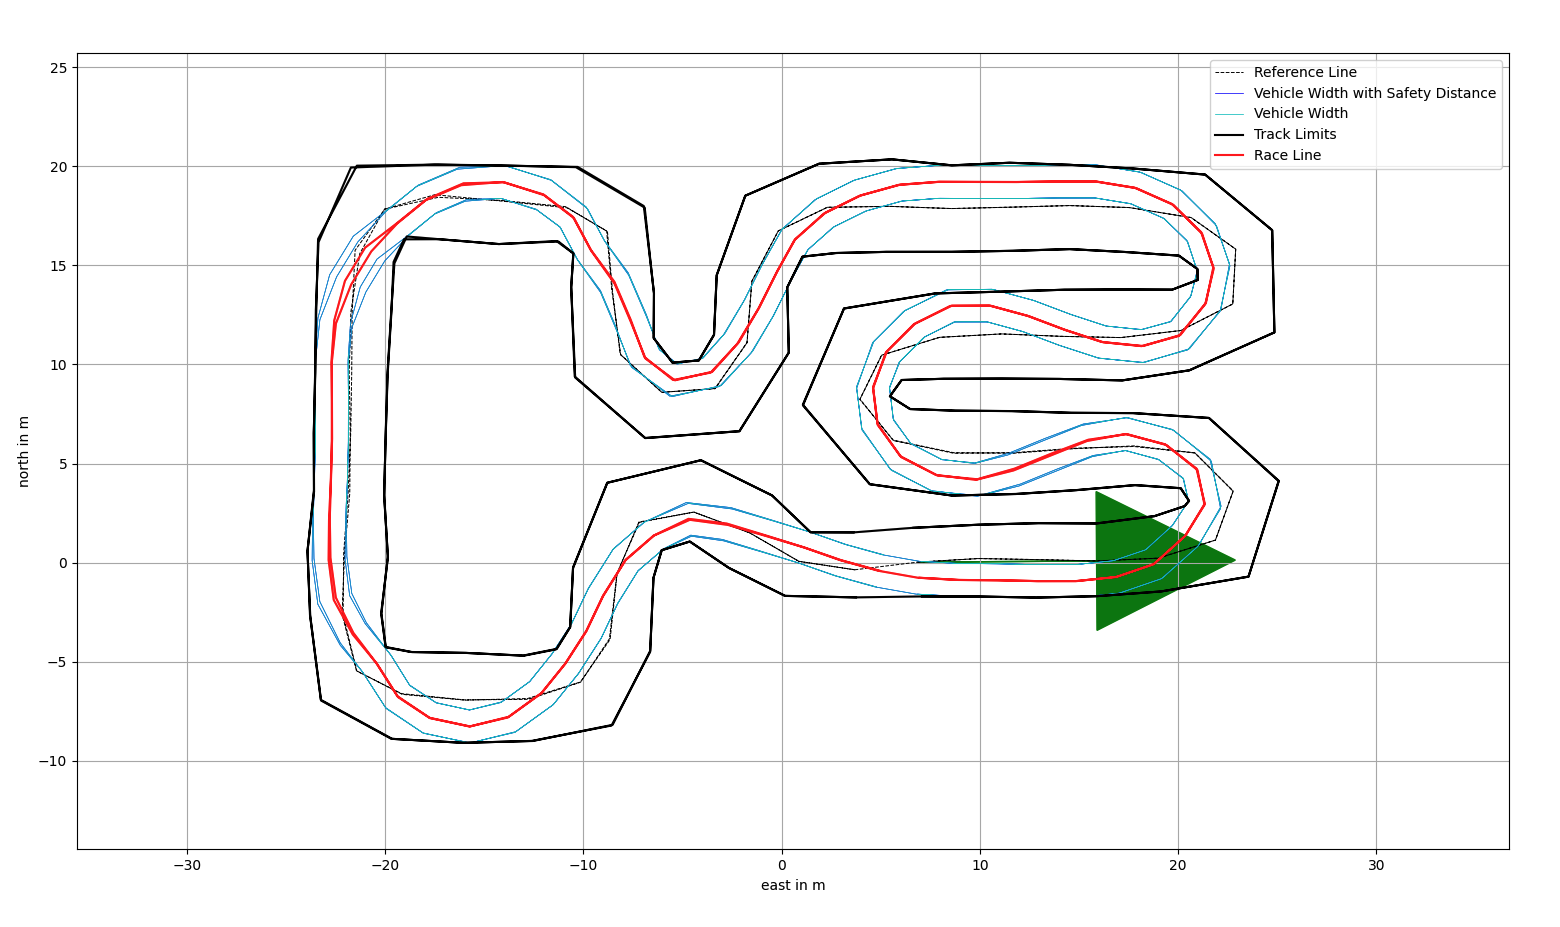
\includegraphics[width=\columnwidth]{Results_Optimization_Garden_Light_Laps_2.png}
    \caption{Optimization on the Garden Light Track for two laps.}
    \label{fig:Results Garden Light Laps 2}
\end{figure}

Another track used for testing the final implementation was the ``Garden Light'' track. The track has some parts where the left track limits (blue cones) are very close. Additionally, the track has additional cones on its curves. The final result on this track can be seen in figure \ref{fig:Result Garden Light Final}.
\begin{figure}[H]
    \centering
    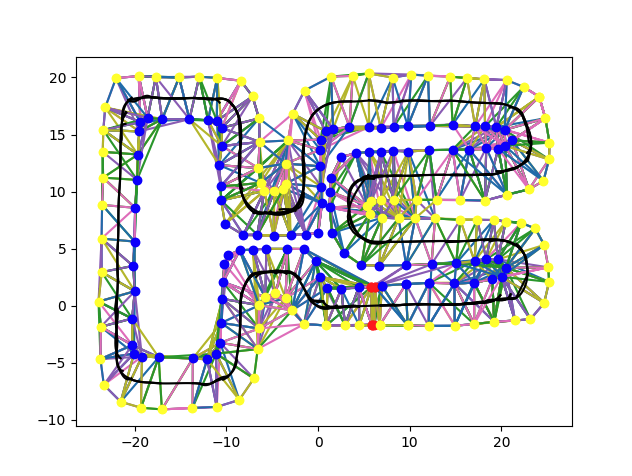
\includegraphics[width=\columnwidth]{Result_GardenLight_final.png}
    \caption{The result of the final exploration algorithm applied on the ``Garden Light`` track.}
    \label{fig:Result Garden Light Final}
\end{figure}

\textbf{Following Tracks are Optimization only!}

\section{Rounded Rectangle Track} \label{sec:Results Rounded Rectangle Track}
Rounded Rectangle:
mincurv 0.39s 36.18s 310p
shortest 0.32s 38.39s 293p
iqp 0.59s 31.28s 303p

\begin{figure}[H]
    \centering
    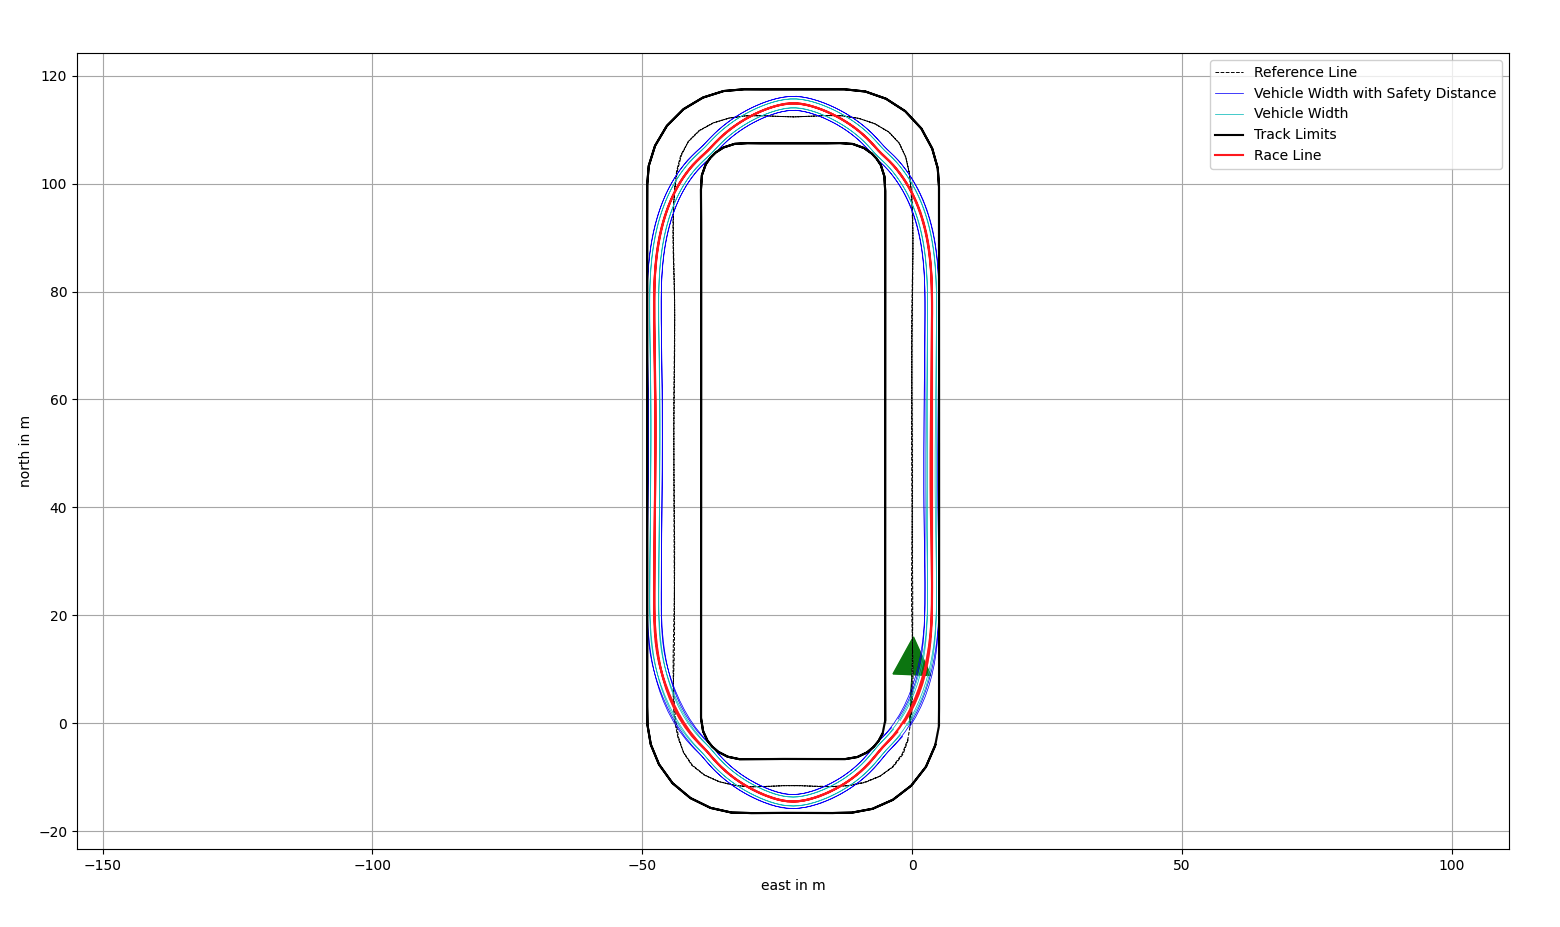
\includegraphics[width=\columnwidth]{Results_Optimization_Rounded_Rectangle_Laps_2.png}
    \caption{Optimization on the Rounded Rectangle Track for two laps.}
    \label{fig:Results Rounded Rectangle Laps 2}
\end{figure}

\section{Handling Track} \label{sec:Results Handling Track}
Handling Track:
mincurv 1.72s 71.94s 582p
shortest 1.15s 74.79s 563p
iqp 3.59s 67.95s 587

\begin{figure}[H]
    \centering
    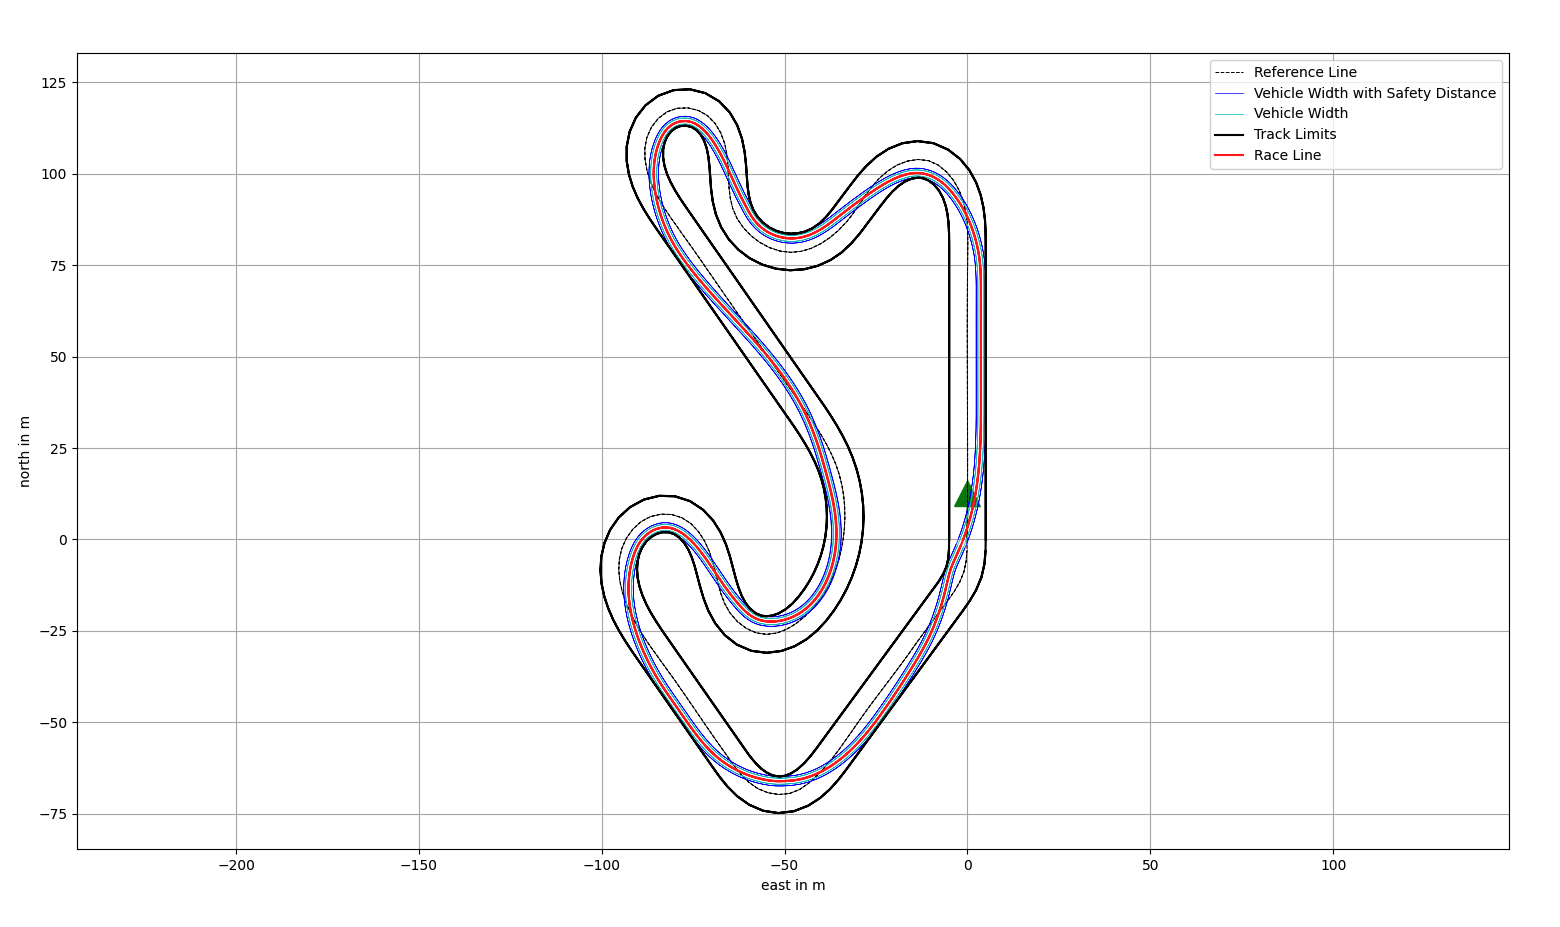
\includegraphics[width=\columnwidth]{Results_Optimization_Handling_Track_Laps_2.png}
    \caption{Optimization on the Handling Track for two laps.}
    \label{fig:Results Handling Track Laps 2}
\end{figure}

\section{Berlin 2018 Track} \label{sec:Results Berlin 2018 Track}
All 2 Laps
Berlin 2018:
mincurv 38.30s 186.15s 2325p
shortest 23.03s 196.57s 2272p
iqp 102.86s 184.00s 2322p

\begin{figure}[H]
    \centering
    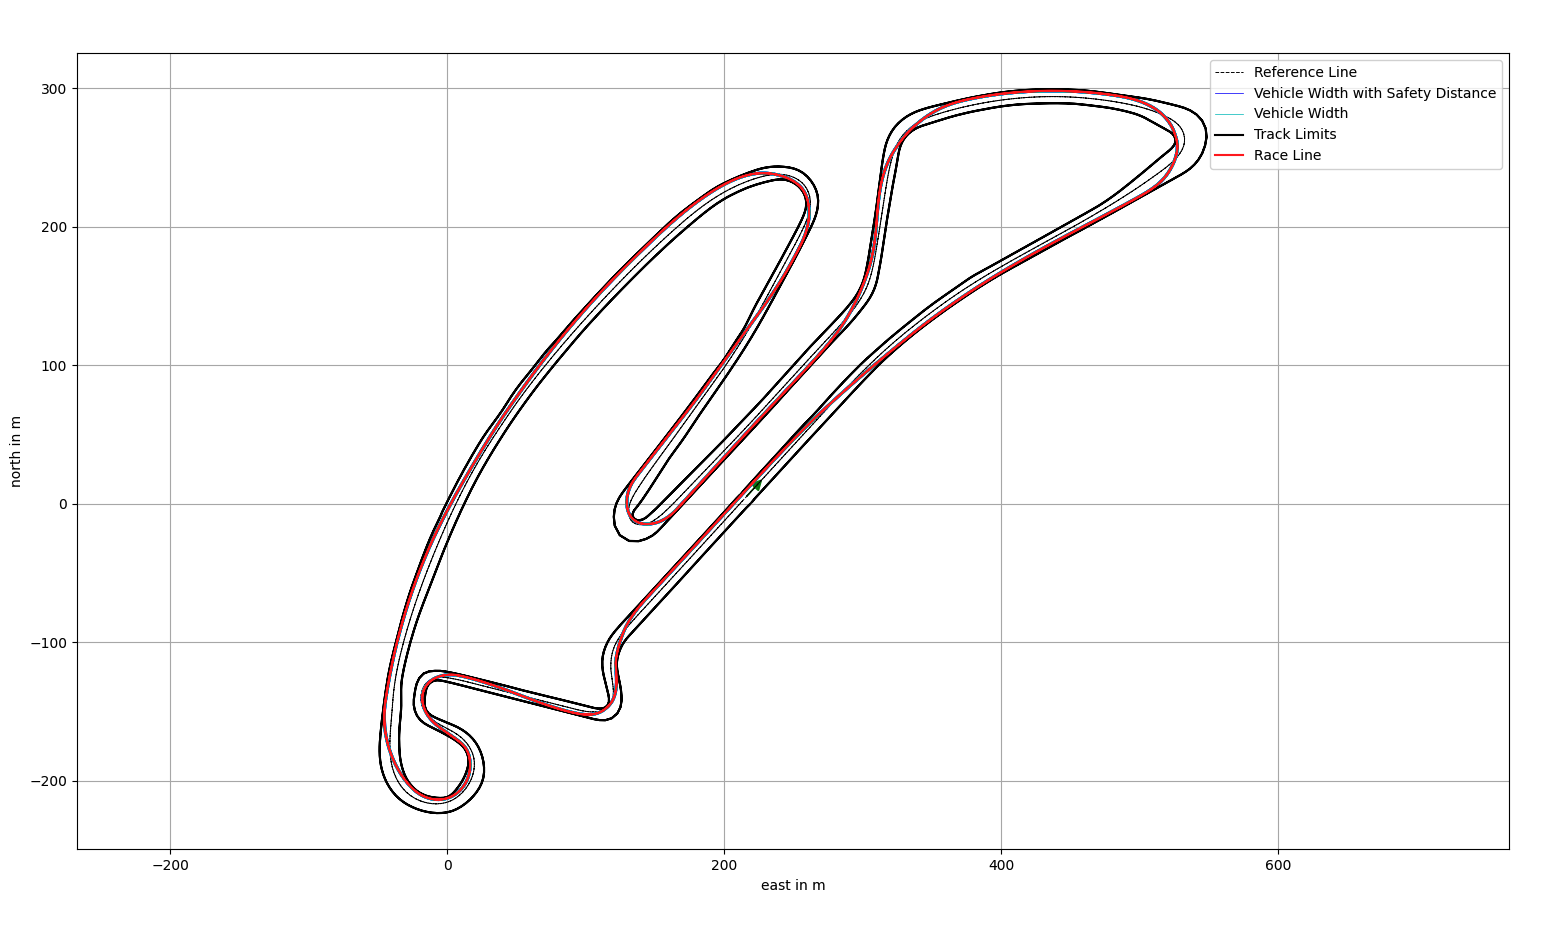
\includegraphics[width=\columnwidth]{Results_Optimization_Berlin_2018_Laps_2.png}
    \caption{Optimization on the Berlin 2018 Track for two laps.}
    \label{fig:Results Berlin 2018 Laps 2}
\end{figure}

Optimization times for berlin\_2018
shortest\_path = 16.72s
Estimated lap time: 89.12s
mincurv = 44.40s
Estimated lap time: 82.46s
mincurv\_iqp = 127.69s
Estimated lap time: 81.06s
mintime = 92.00s
Estimated lap time: 85.77s

\section{Modena 2019 Track} \label{sec:Results Modena 2019 Track}
Modena 2019:
mincurv 26.00s 171.20s 1998p
shortest 14.51s 184.03s 1946p
iqp 69.75s 169.11s 1998p

\begin{figure}[H]
    \centering
    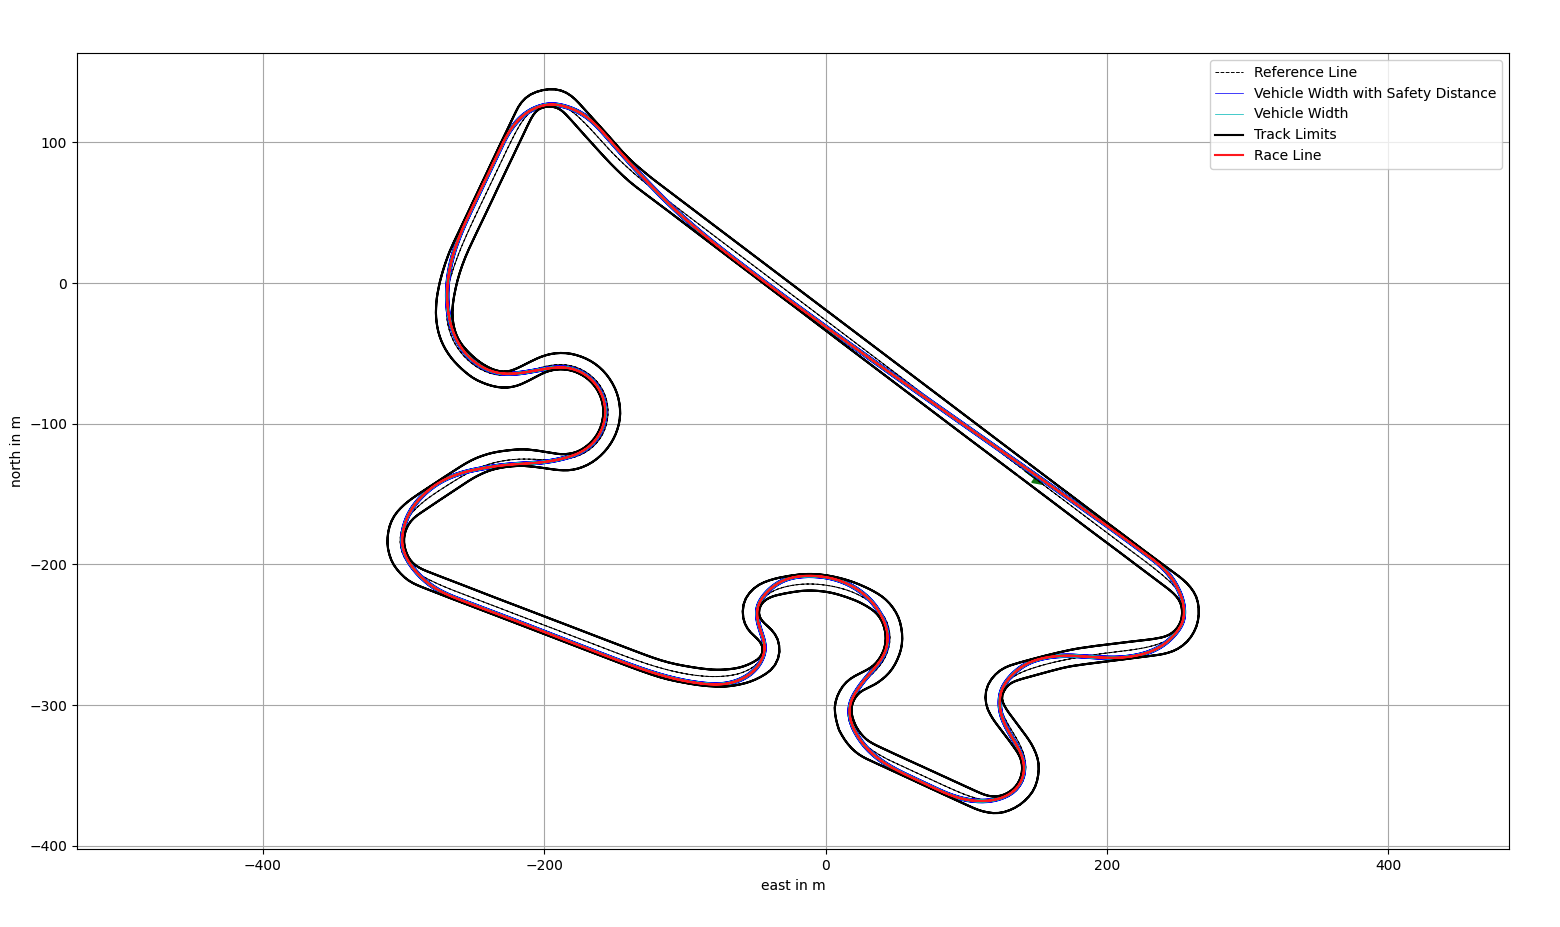
\includegraphics[width=\columnwidth]{Results_Optimization_Modena_2019_Laps_2.png}
    \caption{Optimization on the Modena 2019 Track for two laps.}
    \label{fig:Results Modena 2019 Laps 2}
\end{figure}

\section{Integration}
\begin{itemize}
    \item Test im Python Plots
    \item Simulationstool (Screenshot, evtl. folge von Screenshots), welche strecke (grafik simulationstool)
\end{itemize}

